\documentclass[fleqn,usenatbib,twocolumn]{mnras}
\usepackage[utf8]{inputenc}
\usepackage{graphicx}
\usepackage{mathtools}
\usepackage{siunitx}
\usepackage{enumerate}
\usepackage{caption,subcaption}
\usepackage{comment}
\captionsetup{compatibility=false}
\usepackage{animate}
\usepackage{amsmath} % For \text and many other math symbols
\usepackage{amssymb} % For \mathbb
\usepackage{amsfonts} % For \mathbb


\newcommand{\abs}[1]{\left|#1\right|}
\newcommand{\norm}[2]{\left\lVert#1\right\rVert}

\title{Generative AI for Image Reconstruction with Intensity Interferometry: A First Attempt}
\date{}

\begin{document}
\maketitle

\begin{abstract}
In modern astronomy, simulation and observation with Intensity Interferometry (II) are showing noteworthy progress with optical wavelengths to achieve high-resolved stellar objects. Despite these achievements, phase retrieval of the signal remains challenging due to photon correlation, hence the image reconstruction. Here, we propose the application of a conditional Generative Adversarial Network (cGAN) to II simulated data to overcome the limitations of traditional image reconstruction methods, as Artificial Intelligence (AI) techniques are at the forefront of revealing astronomical mysteries by analyzing the signal. Here, the cGAN effectively reconstructs the shape, size, and brightness distribution of a fast-rotating star by utilizing sparsely sampled, phase-subtracted Fourier transforms of the star. Simulations of II are based on an assembly of four telescopes similar to existing arrays. However, the sensitivity of the signal and high resolution are expected to improve with additional baselines, which makes the current and future Cherenkov Telescope Array Observatory (CTAO) an ideal candidate for II applications. This approach is highly relevant to the existing image reconstruction technique with II and could revolutionize high-resolution imaging in astronomy.
\end{abstract}
\section{Introduction}

Intensity Interferometry (II) emerged in the 1970s as a groundbreaking technique for measuring the diameters, orbits, and limb-darkening coefficients of 32 stars in the N-body system. Despite these significant achievements, the method did not gain widespread adoption due to the then-required highly sensitive photon detectors and sophisticated data analysis techniques. However, advancements in computational methods and modern electronics, which now offer time resolution of detectors in the nanoseconds (ns) to picoseconds (ps) range, have renewed II as a feasible technique for resolving astrophysical objects at visible wavelengths. Current simulations with ns resolution of photon detectors show that II is effective in achieving high precision measurement of parameters for stellar objects \citep{10.1093/mnras/stab2391, 10.1093/mnras/stac2433}. However, a significant drawback of II is the loss of phase information. Consequently, a full reconstruction of the brightness distribution of a source with II necessitates phase information.

Several theoretical and computational approaches to phase reconstruction with II have been proposed. \cite{gamo1963triple} introduced the concept of triple-intensity correlation, which \cite{goldberger1963use} further applied in an experiment to observe scattered particles in microscopic systems. Sato conducted experiments to measure the diameter and phase of asymmetrical objects, suggesting that triple correlation could extend II to image stellar bodies \citep{sato1978imaging, sato1979computer, sato1981adaptive}. Despite its potential, the sensitivity of the signal to noise poses a significant challenge for this approach.

Later \cite{holmes2010two} proposed an alternative method, utilizing the Cauchy-Riemann relations to reconstruct 1-D images and extending this to 2-D images across a range of signal-to-noise (SNR) values. This algorithm was applied to simulated data of stellar objects using II, considering existing and forthcoming Imaging Cherenkov Telescope Arrays (IACTs) with a large number of telescopes \citep{nunez2010stellar, nunez2012high, nunez2012imaging}.

In this paper, we propose an alternative approach using Generative Adversarial Networks (GANs) \citep{goodfellow2014generative} to reconstruct images of stellar objects using II. We consider four Imaging Cherenkov Telescope Arrays (IACTs) located in the Northern Hemisphere and perform a one-night simulation for a fast-rotating star. The predicted image using a trained GAN shows promising results for reconstructing the image's shape and size. The evaluation of the predicted image is conducted using image moments, demonstrating that the size and shape of the fast-rotating star are reconstructed. However, the brightness distribution recovers only at the third-order moment.

This paper is organized as follows: The first section discusses Intensity Interferometry following its signal and noise for fast-rotating stars along the Earth's rotation. The second section introduces the GAN formulation and its structure. Following the third section details the parameter selection for training the GAN to reconstruct the image. After that, the fourth section presents the results of trained GAN visually and using image moments. At the end, there is a discussion of the entire result.
\section{Intensity Interferometry with Imaging Cherenkov Telescope Array}
Recently, Intensity Interferometry (II) has emerged again as an additional tool to resolve stellar objects as it solves some of the key limitations of classical optical interferometry (atmospheric turbulence, length of baseline, and the sensitivity of the optical aperture). It is suitable for the high-resolution study of very massive, hot, and short-lived stars, such as OB-type, Wolf-Rayet, and Pulsating stars in N-body systems. R. Hanbury Brown and Robert Q. Twiss first installed the Narrabri Stellar Intensity Interferometer (NSII) in 1974 to resolve the diameter of bright stars at visible wavelengths \citep{brown1954lxxiv, brown1974intensity}. Nowadays, Imaging Cherenkov Telescope Arrays (ICTAs), which are primarily used for gamma-ray observations, are at the forefront of implementing II during moonlit nights when it does not detect gamma-ray radiation. As a result, detection of intensity correlation and angular size measurements of stars is going on for highly resolved imaging with optical wavelength, particularly using Very Energetic Radiation Imaging Telescope Array Systems (VERITAS), High Energy Stereoscopic Systems (HESS), and Major Atmospheric Gamma Imaging Cherenkov Telescopes (MAGIC) \citep{kieda2022performance, zmija2022optical, abe2024performance}.

\subsection{The signal for II}\label{sec:signal}
In a simple case, an II consists of two light collectors, for example, MAGIC-I and MAGIC-II, which are pointed to a star and measure the intensity $I_1(t)$ and $I_2(t)$ respectively \citep{acciari2020optical, dravins2013optical}. The signals from both detectors are cross-correlated and averaged over time, which results in an equation form
\begin{equation}
	g^{(2)} = \frac{\left\langle I_1(t) \cdot I_2(t + \tau) \right\rangle}{\langle I_1(t) \rangle \cdot \langle I_2(t) \rangle} 
	\label{eqn:HBT}
\end{equation}
where $\tau$ is the time delay between both telescopes. If the light source is chaotic and randomly polarized, we have:
\begin{equation}
	g^{(2)} = 1 + \frac{\Delta f}{\Delta \nu} \abs{V_{12}}^2
	\label{eqn:HBT2}
\end{equation}
here, $\Delta f$ is the electronic bandwidth, $\Delta \nu$ is the optical bandwidth, and $\Delta f \ll \Delta \nu$ \citep{acciari2020optical}. $V_{12}$ is the Fourier transform of the source brightness distribution and is called complex visibility. Eqn.~\ref{eqn:HBT2} carry the information about the source's structure and shape. However, it loses the phase information due to the presence of only the absolute value of $V_{12}$. In observational astronomy, the correlation in intensity is often expressed in terms of the normalized contrast, given by :
\begin{equation}
	c = \frac{\left\langle \left( I_1(t) - \left\langle I_1 \right\rangle \right) \cdot \left( I_2(t + \tau) - \left\langle I_2 \right\rangle \right) \right\rangle}{\langle I_1(t) \rangle \cdot \langle I_2(t) \rangle} = g^{(2)} - 1
\end{equation}
where, $\left\langle I_1 \right\rangle$ and $\left\langle I_2 \right\rangle$ are the mean intensity from two telescopes.

\subsection{Signal-to-Noise Ratio for Intensity Interferometry}
\begin{figure}
	\centering
	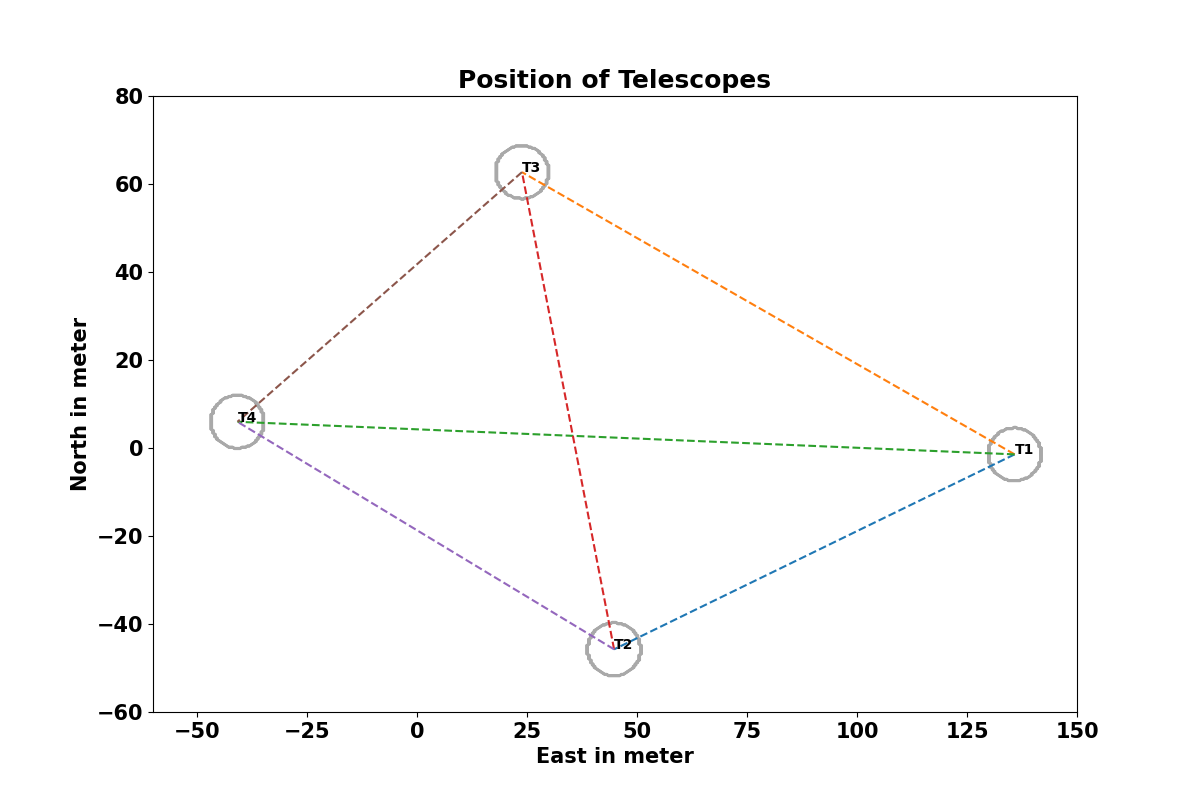
\includegraphics[width=\linewidth]{fig/telescope.png}
	\caption{Configuration of the four Imaging Cherenkov Telescope Array (ICTAs) with similar properties each used to simulate the signal for II.}
	\label{fig:teles}
\end{figure}
The main physics channel of ICTAs is the study of Very High Energy gamma rays ($\geq 30$ GeV) originating from particle showers in the atmosphere. Telescopes have an array of mirrors, which focus the light onto an array of photo-multiplier tubes (PMTs) \citep{aleksic2016major}. Here, Fig.~\ref{fig:teles} shows an arrangement of four ICTAs with similar properties each. For the simulation of II, the light of a stellar source is focused on a single PMT, which has a filter in front. The purpose of this filter is to efficiently transmit light around mean observational frequency, which protects the PMTs from excessive light. It is necessary, as II observations are mainly done during full moon nights when it is too bright for Very High Energy $\gamma$-ray observations. The optical signal of the PMTs is transmitted with optical fibers, converted to an electrical signal, and digitized \citep{acciari2020optical}. The measurable observable is the Pearson's correlation coefficient:
\begin{equation}
	\rho(\tau) = \frac{\left\langle \left( I_1(t) - \left\langle I_1 \right\rangle \right) \cdot \left( I_2(t + \tau) - \left\langle I_2 \right\rangle \right) \right\rangle}{\sqrt{\langle \left( I_1(t) - \langle I_1 \rangle \right)^2 \rangle} \cdot \sqrt{\langle \left( I_2(t) - \langle I_2 \rangle \right) ^2 \rangle}}
	\label{eqn:pearson}
\end{equation}
It must be noted that the calculation of Pearson's correlation coefficient is non-trivial: MAGIC makes use of the convolution theorem for discrete Fourier transforms because it is computationally more efficient. Since $I_1$ and $I_2$ are proportional to the direct current of the PMTs ($DC_i$), the normalized contrast can be calculated as 
\begin{equation}
	c \propto \frac{\rho}{\sqrt{\left(DC_1 \cdot DC_2 \right)}}.
	\label{eq:norm_contrast2}
\end{equation}
One must also correct for a non-constant gain of the PMTs, as well as the moon. The latter can be done by measuring the background light with an additional PMT with no mirrors focused on it \citep{acciari2020optical}.

The significance of the signal is expressed as the signal-to-noise ratio (SNR), which depends on many factors. However, most importantly, SNR is proportional to the absolute value of visibility, which itself depends on the distance between the telescopes \citep{acciari2020optical} 
\begin{equation}
	SNR = A \cdot \alpha \cdot q \cdot n \cdot \abs{V_{12}}^{2}(d) \cdot \sqrt{b_v} \cdot F^{-1} \cdot \sqrt{\frac{T}{2}} \cdot \sigma.
	\label{eq:SNR}
\end{equation}
Here, $A$ is the total mirror area, $\alpha$ the quantum efficiency of the PMTs, $q$ the quantum efficiency of the optics, $n$ the differential photon flux from the source, and $b_v$ the cross-correlation bandwidth. The noise of the PMTs is accounted with $F$, $T$ denotes the observation time, and $\sigma$ is the normalized spectral distribution of the light (including filters) \citep{acciari2020optical}. While most of the parameters can be optimized with hardware, the only way to obtain a better SNR is to increase the observation time with a fixed number of telescopes.  
\begin{figure}
	\centering
	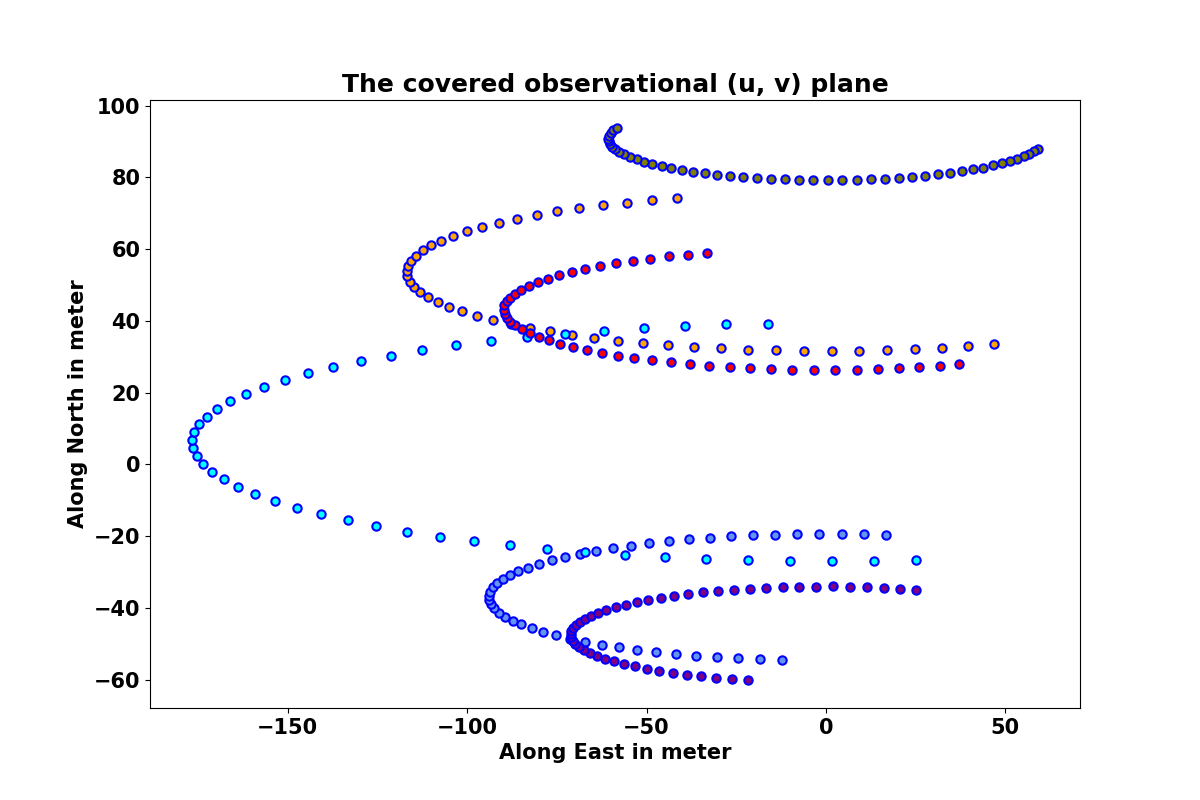
\includegraphics[width=\linewidth]{fig/baseline.png}
	\caption{The tracking of baselines with four telescopes arranged in fig.~\ref{fig:teles} for one night of observation.}
	\label{fig:base}
\end{figure}
\begin{figure}
	\centering
	
\includegraphics[width=0.8\linewidth]{fig/ellipse/ellipse6018.jpg}
	\caption{This figure shows one of the simulated fast-rotating stars. The brightness is highest at the pole and lowest at the equator due to the presence of high-speed rotation of the star. This effect is named gravitational darkening in astronomy.}
	\label{fig:image}
\end{figure}
\subsection{Baseline considerations}
The measurement of the size of stellar objects through absolute visibility depends on the distance between the telescopes, which is called the baseline $B$
\begin{equation}
	V_{12}(B) = \frac{c(B)}{c(0)}.
	\label{eq:angular_size_meas}
\end{equation}
However, this work needs a good SNR value for high precision of measurement, so the large covered observational plane with telescopes is a necessity for II \citep{acciari2020optical, abeysekara2020demonstration}. If the source is at the zenith, the coordinates in the Fourier plane ($u,v$) are given by:
\begin{equation}
	(u,v) = \frac{1}{\lambda} (B_N, B_E)
\end{equation}
where $B_N$ and $B_E$ are the baselines expressed in north and east coordinates. Since not all sources are at the zenith, and the telescopes are stationary, Earth's rotation plays an important role in covering the maximum observational plane through the rotated baselines, which is given as  
\begin{equation}
	\begin{pmatrix} u\\ v\\ w\\ \end{pmatrix} = R_x(\delta) \cdot R_y(h) \cdot R_x(-l) \begin{pmatrix} B_N\\ B_E\\ B_A\\ \end{pmatrix}
	\label{eq:baseline_rot}
\end{equation}
It traces an ellipse for every pair of telescopes. Furthermore, the different altitudes of the telescopes $B_A$ must be considered \citep{dravins2013optical, saha2020theory}. Here, $\delta$ is the declination, and $h$ is the hour angle of the stellar source, and $l$ is the latitude of the telescopes. The three matrices $R_i$ correspond to the fundamental representation of the SO(3) group \citep{saha2020theory}. Fig.~\ref{fig:base} shows the track of six baselines generated from the telescopes (fig.~\ref{fig:teles}) due to Earth's rotation. Since every pair of telescopes traces an ellipse in the Fourier plane, the total number of ellipses scales as follows:
\begin{equation}
	\label{eq:N_telescopes}
	\mathcal{N} = \frac{N_T \cdot (N_T -1)}{2}
\end{equation}

As the number of baselines increases non-linearly, II benefits greatly from a large number of telescopes. The existing and upcoming Cherenkov Telescope Array Observatory (CTAO) can promise to cover the maximum observational plane and provide insight into stellar objects with optical wavelengths in the future.
\begin{figure}
	\centering
	\begin{subfigure}{\linewidth}
		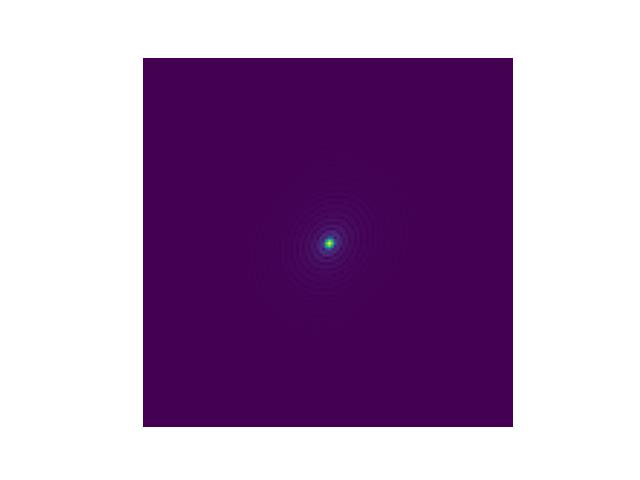
\includegraphics[width=\linewidth]{fig/ft/ft.jpg}
		\caption{The Fourier transform of the source.}
	\end{subfigure}\hfill
	\begin{subfigure}{\linewidth}
		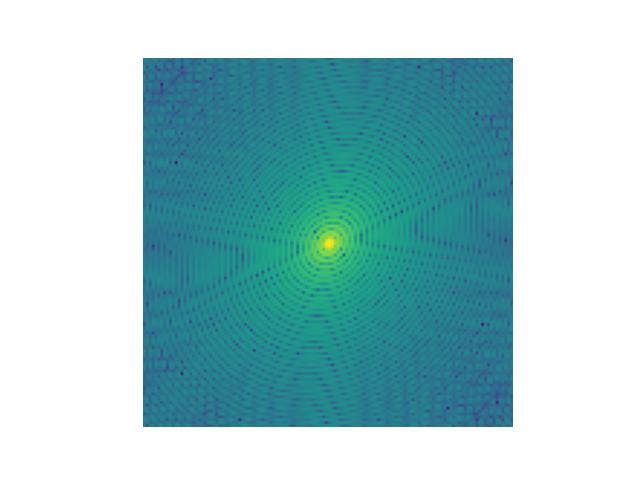
\includegraphics[width=\linewidth]{fig/ft/ft_log.jpg}
		\caption{The logarithmic Fourier transform of the source.}
	\end{subfigure}
	\caption{Absolute value of the two-dimensional Fast Fourier Transform of Fig.~\ref{fig:image} on linear and logarithmic scales. Observation of the maximum (u, v) plane with a finite number of baselines can be completed with the help of Earth's rotation.}
	\label{fig:ft}
\end{figure}
\begin{figure}
	\centering
	\begin{subfigure}{\linewidth}
		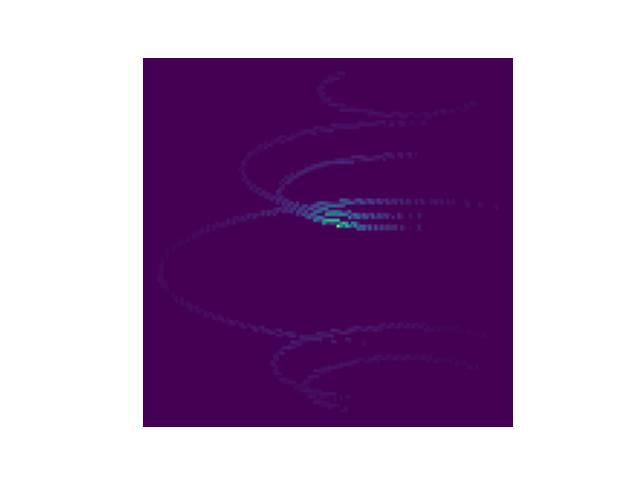
\includegraphics[width=\linewidth]{fig/ft/ft_base.jpg}
		\caption{The Fourier transform with baselines.}
	\end{subfigure}\hfill
	\begin{subfigure}{\linewidth}
		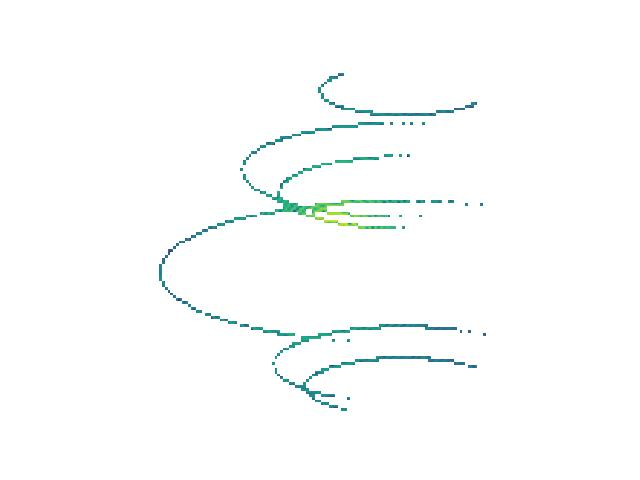
\includegraphics[width=\linewidth]{fig/ft/ft_log_base.jpg}
		\caption{The logarithmic Fourier transform with baselines.}
	\end{subfigure}
	\caption{The upper panel shows the absolute value of the two-dimensional Fast Fourier Transform of Fig.~\ref{fig:image} measured by baselines shown in Fig.~\ref{fig:teles} on a linear scale, and the lower panel shows the same on a logarithmic scale.}
	\label{fig:ft_base}
\end{figure}
\subsection{An Object: Fast Rotating Stars}
In our work, we simulate a single fast-rotating star to test image reconstruction with II in intersection with the Generative Adversarial Networks (GAN). Fast rotation causes stars to take on an oblate shape, flattening at the poles and bulging at the equator due to the existence of stronger centrifugal force \citep{von1924radiative, 1999A&A...347..185M}. Fig.~\ref{fig:image} shows one of the simulations of a fast-rotating star, where the star takes on an elliptical shape with brightness distributed across the object. The brightness is maximum at the poles and minimum at the equator, a phenomenon known as gravity darkening \citep{lucy1967gravity}. This effect was first observed in the fast-rotating star Regulus through interferometric and spectroscopic data from the Center for High Angular Resolution Astronomy (CHARA) Array \citep{mcalister2005first}. These stars are crucial for understanding a variety of astrophysical processes and help to understand the stellar evolution, internal structure, and rotational dynamics over time.

Intensity Interferometry (II) detects the photon from the stellar objects, and the correlation of it results in squared visibility (explained in subsection.\ref{sec:signal}). According to Van Cittert Zernike's theorem, this signal is the Fourier transform of brightness distribution in the sky. Fig.~\ref {fig:ft} visualize this statement for the source shown in Fig.~\ref{fig:image} using II on linear and logarithmic scales. However, current observational techniques are unable to capture the full signal, and only partial data can be collected with a single night's simulation, which has been shown in Fig.~\ref{fig:ft_base}. It is the covered observational plane using the baselines shown in Fig.~\ref{fig:teles} on linear and logarithmic scales, respectively. However, the instrumentation of existing and upcoming CTAO shows the possibility of covering the maximum observable portion of the visibility plane for stellar objects, offering high resolution to understand the stellar structure and its evolution with time.
\section{Generative Adversarial Networks}
Generative Adversarial Networks (GANs) were invented by Ian Goodfellow in 2014. The concept is rather simple, as it consists of two competing networks. The first network is called a generator and creates new images based on an input image. Here, for consistency, the images generated by the generator will be denoted as generated images. The second network is the discriminator, which tries to distinguish between the generated image and the real image (ground truth) \citep{goodfellow2014generative}.
As a consequence of training both networks alternately, the generated images eventually become indistinguishable from the real images. It is nothing more than a two-player min-max game, a famous problem in game theory. GAN was initially proposed in the formulation form as:
\begin{equation}
	\centering
	\begin{aligned}
		\min_{G} \max_{D} V(D, G) &= \mathbb{E}_{x \sim p_{data}(x)} \left[ \log D(x) \right] \\
		&+ \mathbb{E}_{z \sim p_{z}(z)} \left[ \log \left( 1-D(G(z)) \right) \right]
	\end{aligned}
	\label{eq:Basic_GAN}
\end{equation}
here, $V(D, G)$ is the value function of the min-max game. 

The goal is now to learn the distribution of the generator $p_g$ over the data $x$. We have input noise variables $p_z(z)$, as well as the two perceptrons $G(z; \theta_g)$ and $D(x; \theta_d)$ with parameters $\theta_i$. $G$ represents a differential function that maps from $z$ to the data space $x$, while $D(x)$ represents the probability that $x$ is from the real data \citep{goodfellow2014generative}. The problem can be reformulated as: 
\begin{equation}
	\centering
	\begin{aligned}
		\max_{D} V(G, D) &= \mathbb{E}_{x \sim p_{data}} \left[ \log D^{*}_{G}(x) \right] \\ 
		&+ \mathbb{E}_{x \sim p_{g}} \left[ \log \left( 1 - D^{*}_{G}(x) \right) \right]
	\end{aligned}
	\label{eq:GAN_reformulated}
\end{equation}
where $D^{*}_{G}$ denotes the optimum of the discriminator for a given fixed generator and is expressed as
\begin{equation}
	\centering
	D^*_G(x) = \frac{p_{data}(x)}{p_{data}(x) + p_g(g)}
	\label{eq:Disc_optimum}
\end{equation}
It can now be shown that the global optimum of equation (\ref{eq:GAN_reformulated}) is reached if and only if $p_g = p_{data}$. Furthermore, if both $G$ and $D$ are allowed to reach their optima, $p_g$ converges to $p_{data}$. A more detailed discussion of the problem, including proofs, can be found in \citep{goodfellow2014generative}.
\begin{figure}
	\centering
	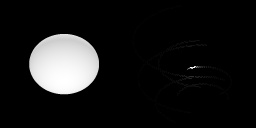
\includegraphics[width=\linewidth]{fig/ellipsoid_0.jpg}
	\caption{Merged image, which includes the original and the sparsely sampled Fourier plane. It is exactly what the GAN receives. }
	\label{fig:GANinput}
\end{figure}
\begin{figure}
	\centering
	\begin{subfigure}{\linewidth}
		\centering
		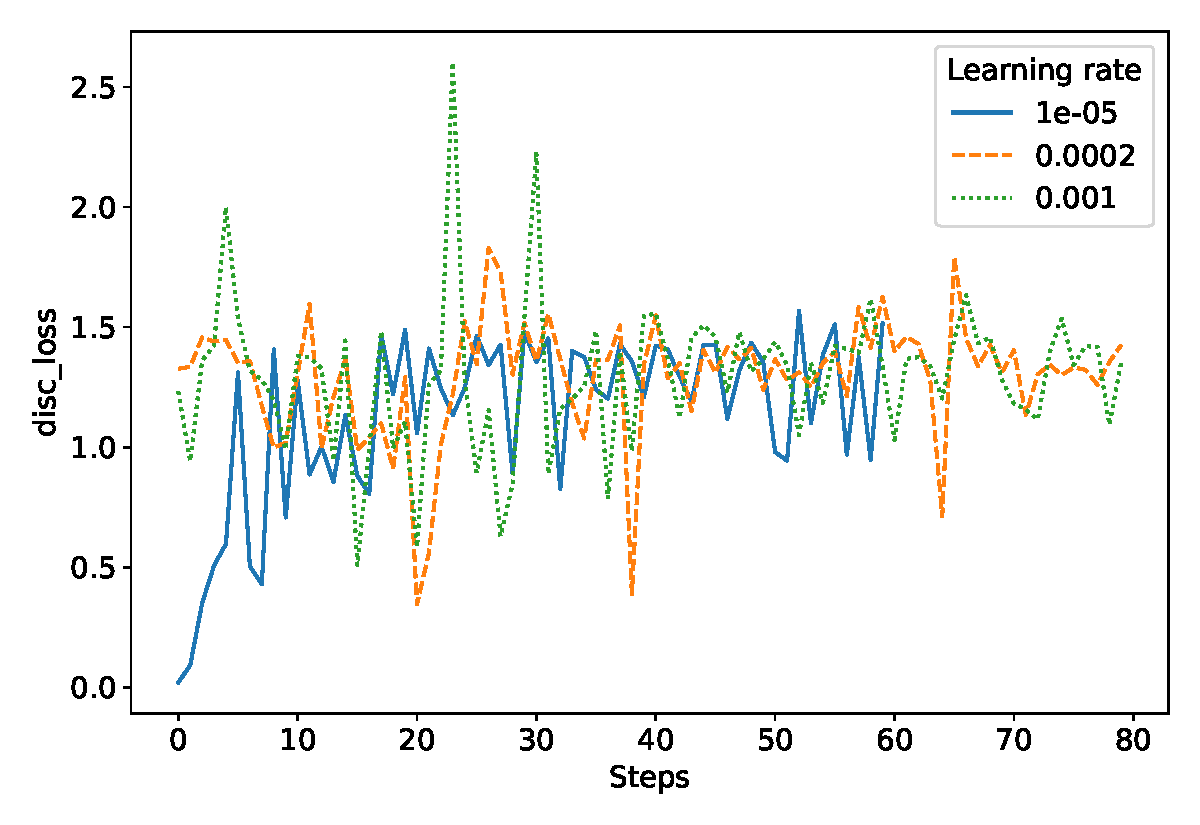
\includegraphics[width=\textwidth]{fig/analysis/Plot_learning_rate_disc_loss.pdf}
		\caption{Discriminator loss for three different learning rates. }
		\label{fig:Plot_learning_rate_discloss}
	\end{subfigure}\hfill
	\begin{subfigure}{\linewidth}
		\centering
		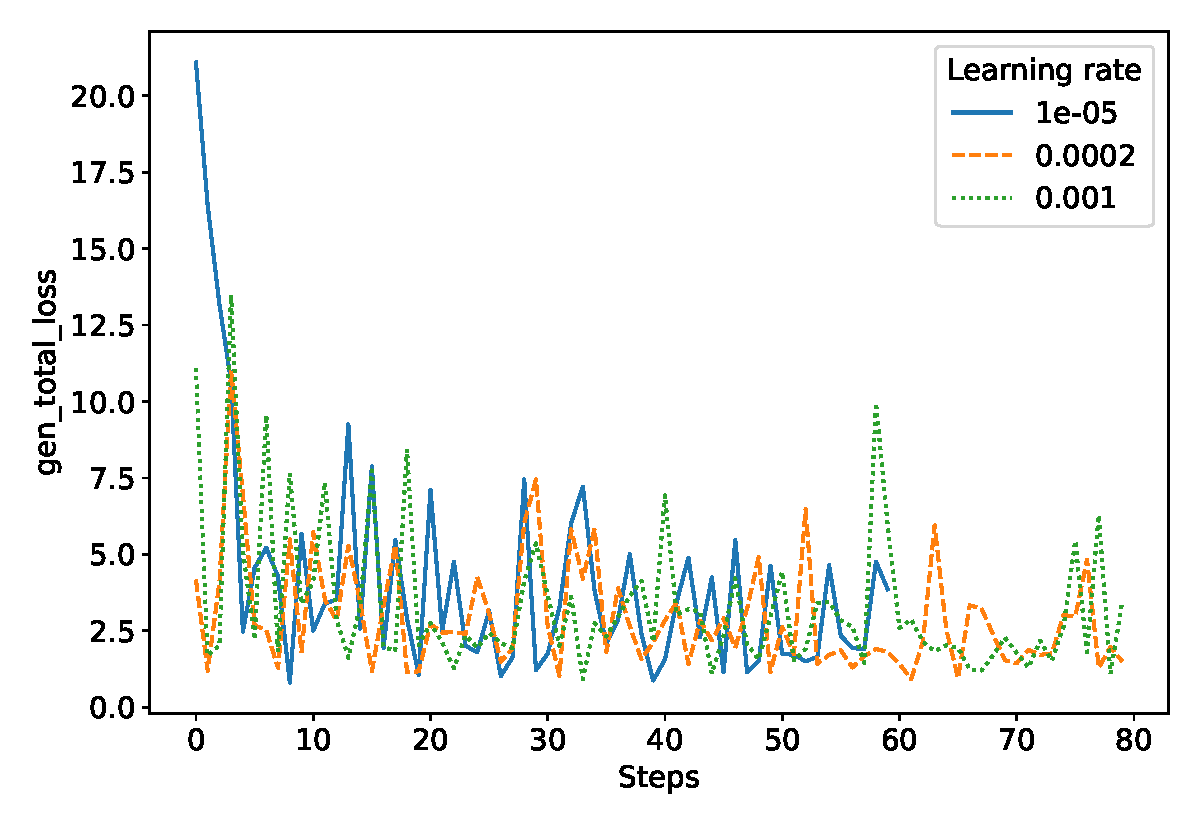
\includegraphics[width=\textwidth]{fig/analysis/Plot_learning_rate_gen_total_loss.pdf}
		\caption{Total generator loss for different learning rates (eqn. (\ref{eq:total_gen_loss})).}
		\label{fig:Plot_learning_rate_genloss}
	\end{subfigure}\hfill
	\caption{Generator and discriminator losses for three different learning rates. The upper figure shows the total discriminator loss, and the lower figure shows the total generator loss. There is no significant difference, but the highest learning rate might be prone to outliers. }
	\label{fig:Plot_learning_rate_loss}
\end{figure}
\begin{figure}
	\centering
	\begin{subfigure}{\linewidth}
		\centering
		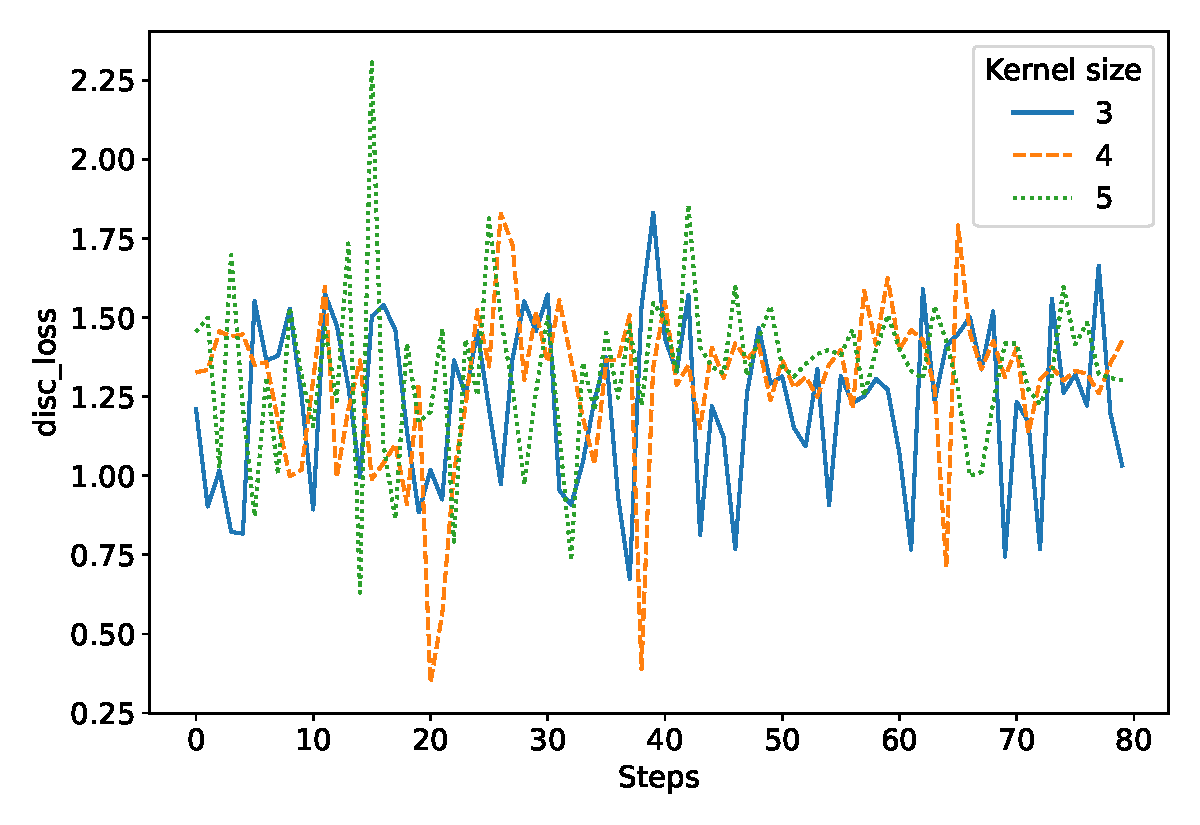
\includegraphics[width=\textwidth]{fig/analysis/Plot_Kernel_size_disc_loss.pdf}
		\caption{Discriminator loss for three different kernel sizes. }
		\label{fig:Plot_kernel_size_discloss}
	\end{subfigure}\hfill
	\begin{subfigure}{\linewidth}
		\centering
		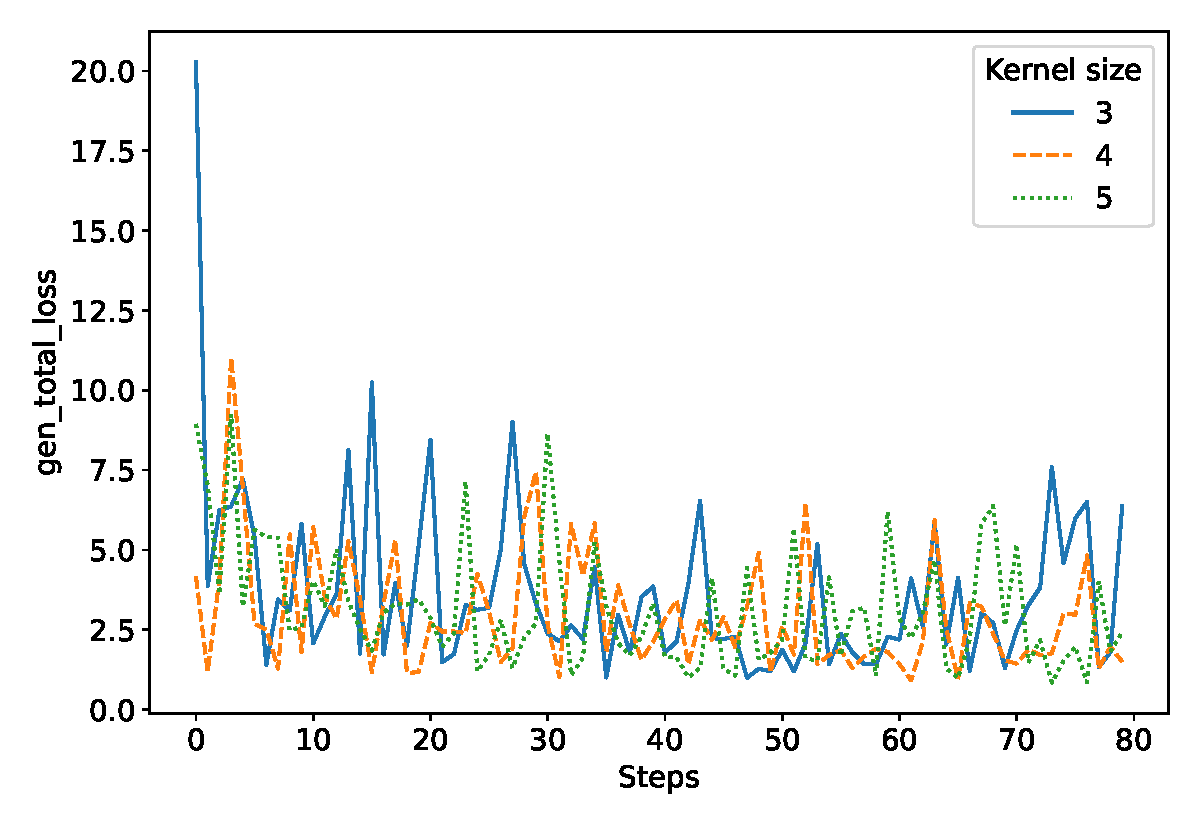
\includegraphics[width=\textwidth]{fig/analysis/Plot_Kernel_size_gen_total_loss.pdf}
		\caption{Total generator loss for three different kernel sizes.}
		\label{fig:Plot_kernel_size_genloss}
	\end{subfigure}\hfill
	\caption{Generator and discriminator losses for three different kernel sizes in the convolutional layers. Here, the smallest kernel size has many outliers, while the largest kernel size seems to be the most stable.}
	\label{fig:Plot_kernel_size_loss}
\end{figure}
\begin{figure*}
	\centering
	\begin{subfigure}{0.5\linewidth}
		\centering
		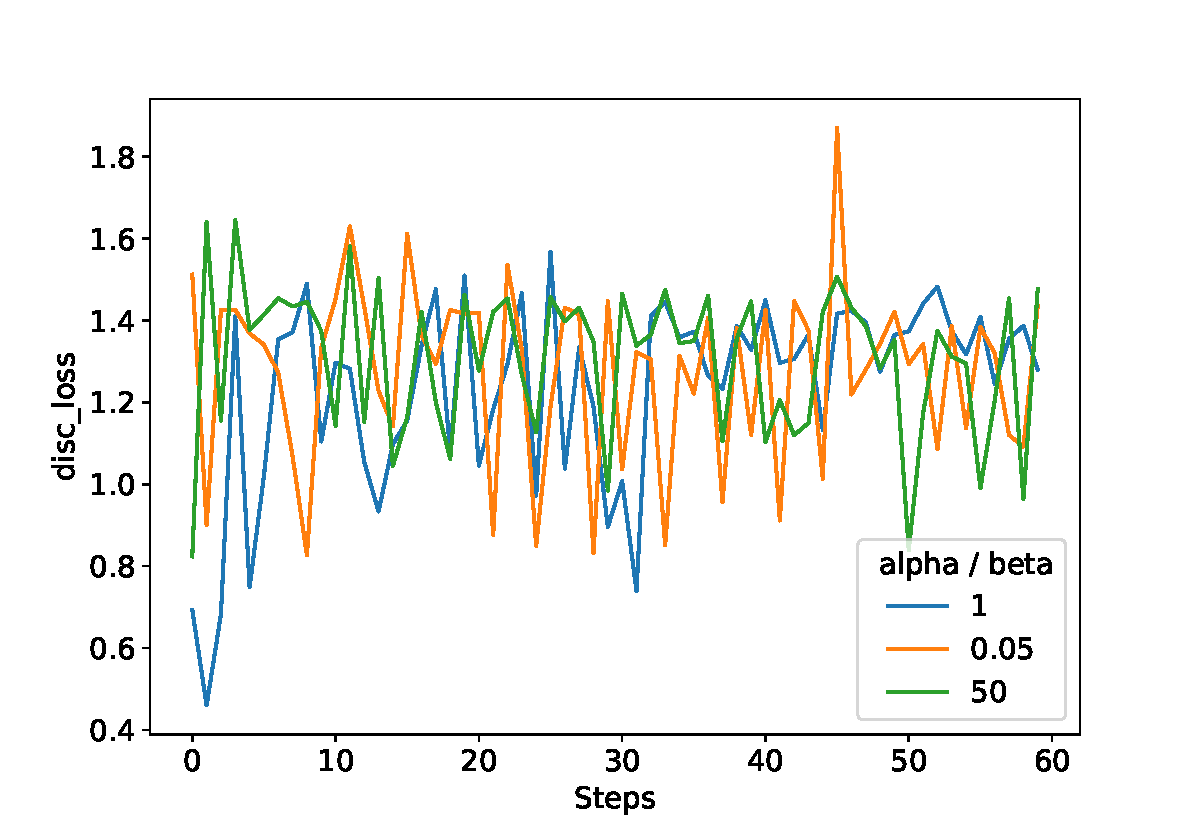
\includegraphics[width=\textwidth]{fig/analysis/Plot_noise_factor_disc_loss.pdf}
		\caption{Discriminator loss for different noise percentages.}
		\label{fig:Plot_noise_discloss}
	\end{subfigure}\hfill
	\begin{subfigure}{0.5\linewidth}
		\centering
		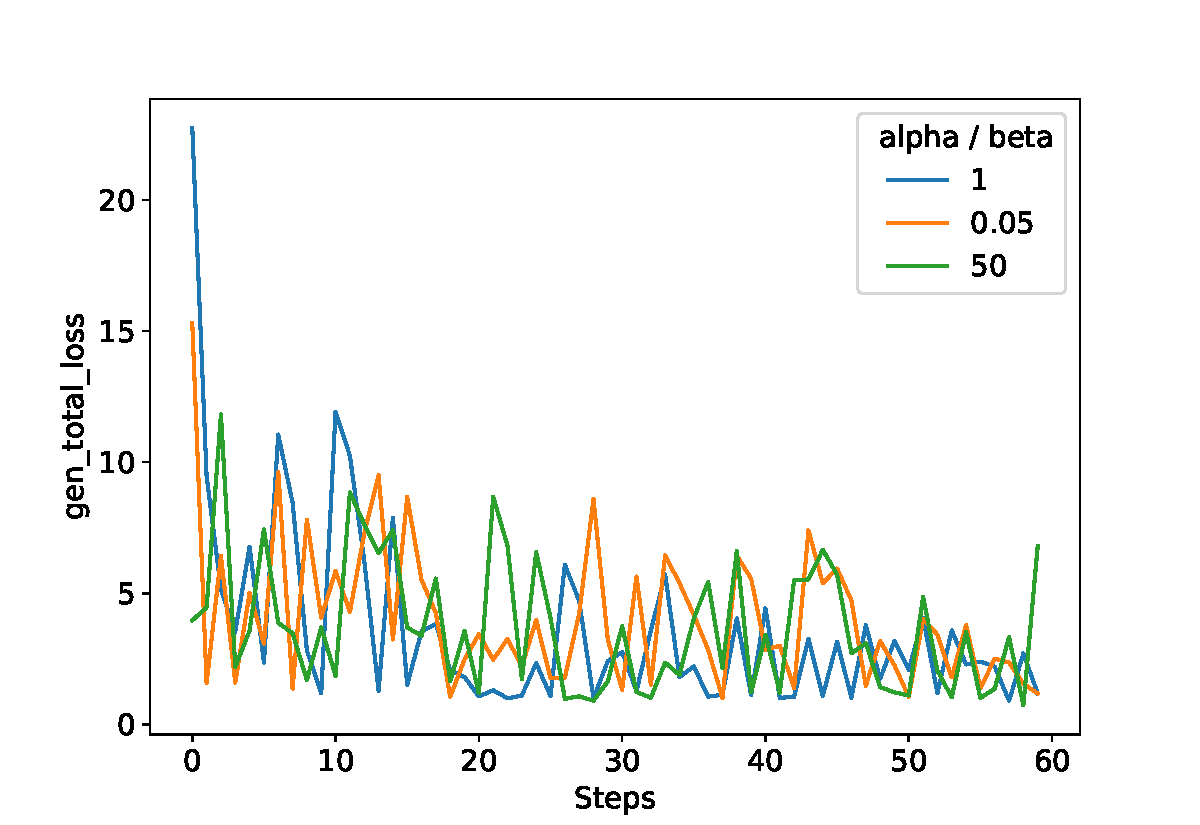
\includegraphics[width=\textwidth]{fig/analysis/Plot_noise_factor_gen_total_loss.pdf}
		\caption{Generator losses for different noise percentages.}
		\label{fig:Plot_noise_genloss}
	\end{subfigure}\hfill
	\caption{Effect of the Salt and Pepper noise introduced in the images. Different ratios between $\alpha$ and $\beta$ are shown. There is no significant effect. Please note that these results are from training on 64-pixel images.}
	\label{fig:Plot_noise_loss}
\end{figure*}
\begin{figure*}
	\centering
	\begin{subfigure}{0.5\linewidth}
		\centering
		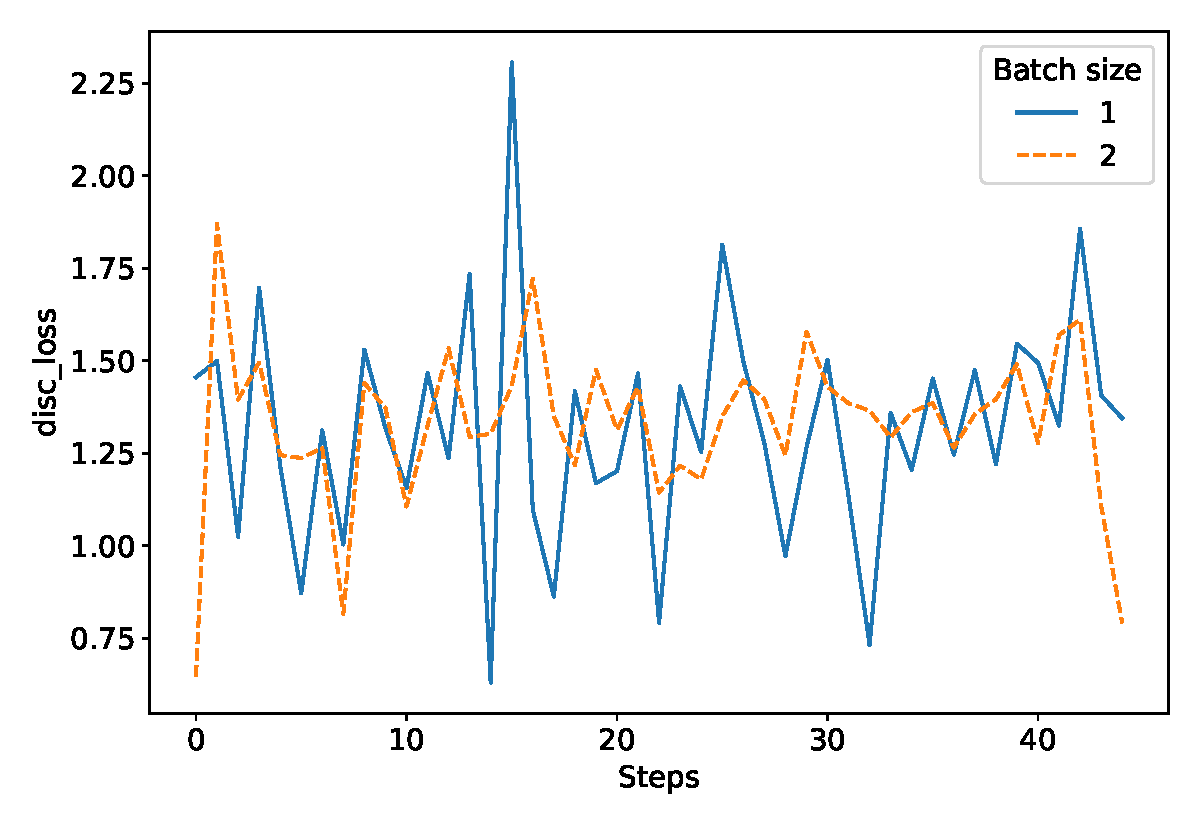
\includegraphics[width=\textwidth]{fig/analysis/Plot_Batchsize_disc_loss.pdf}
		\caption{Discriminator loss for different batch sizes.}
		\label{fig:Plot_batchsize_discloss}
	\end{subfigure}\hfill
	\begin{subfigure}{0.5\linewidth}
		\centering
		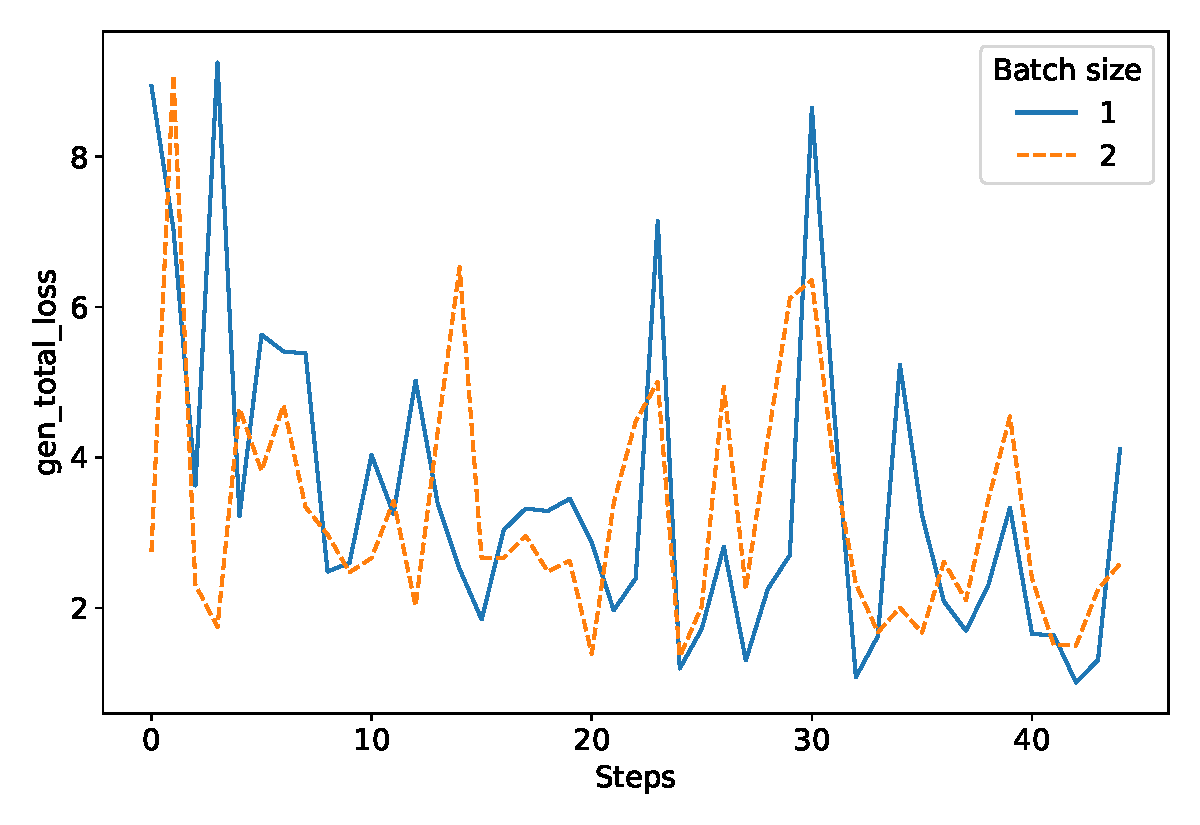
\includegraphics[width=\textwidth]{fig/analysis/Plot_Batchsize_gen_total_loss.pdf}
		\caption{Generator losses for different batch sizes.}
		\label{fig:Plot_batchsize_genloss}
	\end{subfigure}\hfill
	\caption{Loss functions for two different batch sizes. Large batch sizes seem to be more robust, but they also increase training time significantly. }
	\label{fig:Plot_batchsize_loss}
\end{figure*}
\begin{figure*}
	\centering
	\begin{subfigure}{0.5\linewidth}
		\centering
		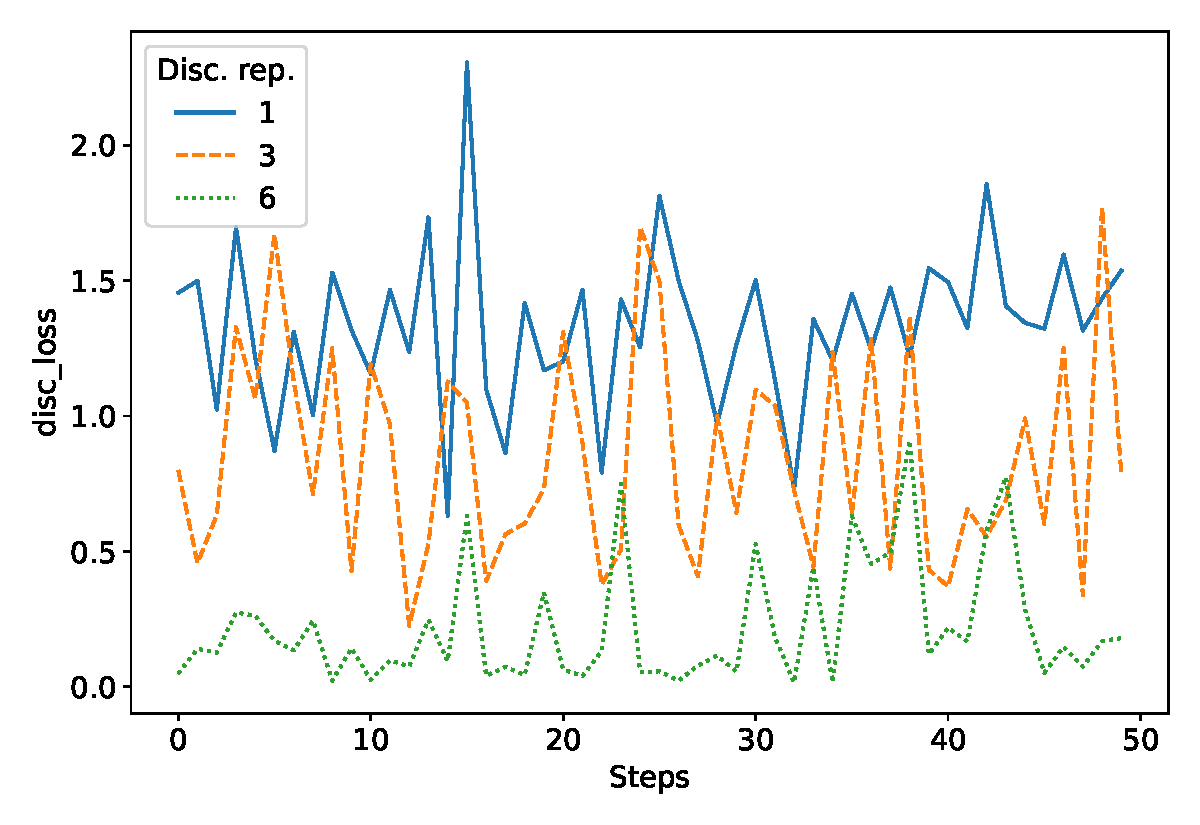
\includegraphics[width=\textwidth]{fig/analysis/Plot_Disc_rep_disc_loss.pdf}
		\caption{Discriminator loss for different discriminator training.}
		\label{fig:Plot_discrep_discloss}
	\end{subfigure}\hfill
	\begin{subfigure}{0.5\linewidth}
		\centering
		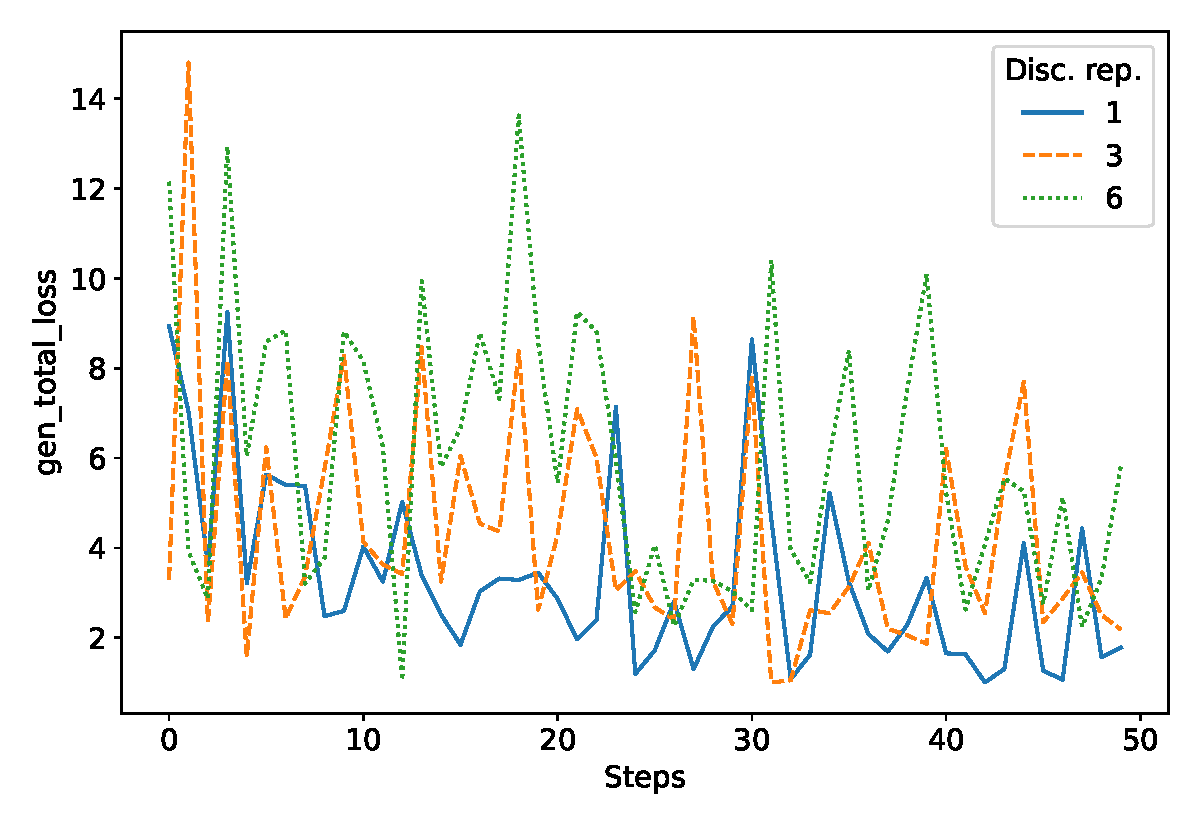
\includegraphics[width=\textwidth]{fig/analysis/Plot_Disc_rep_gen_total_loss.pdf}
		\caption{Generator losses for different discriminator training.}
		\label{fig:Plot_discrep_genloss}
	\end{subfigure}\hfill
	\caption{The amount of discriminator training has a high impact on the discriminator score. The discriminator repetition indicates the factor by which the discriminator is trained more with respect to the generator.}
	\label{fig:Plot_discrep_loss}
\end{figure*}
\begin{figure*}
	\centering
	\begin{subfigure}{0.5\linewidth}
		\centering
		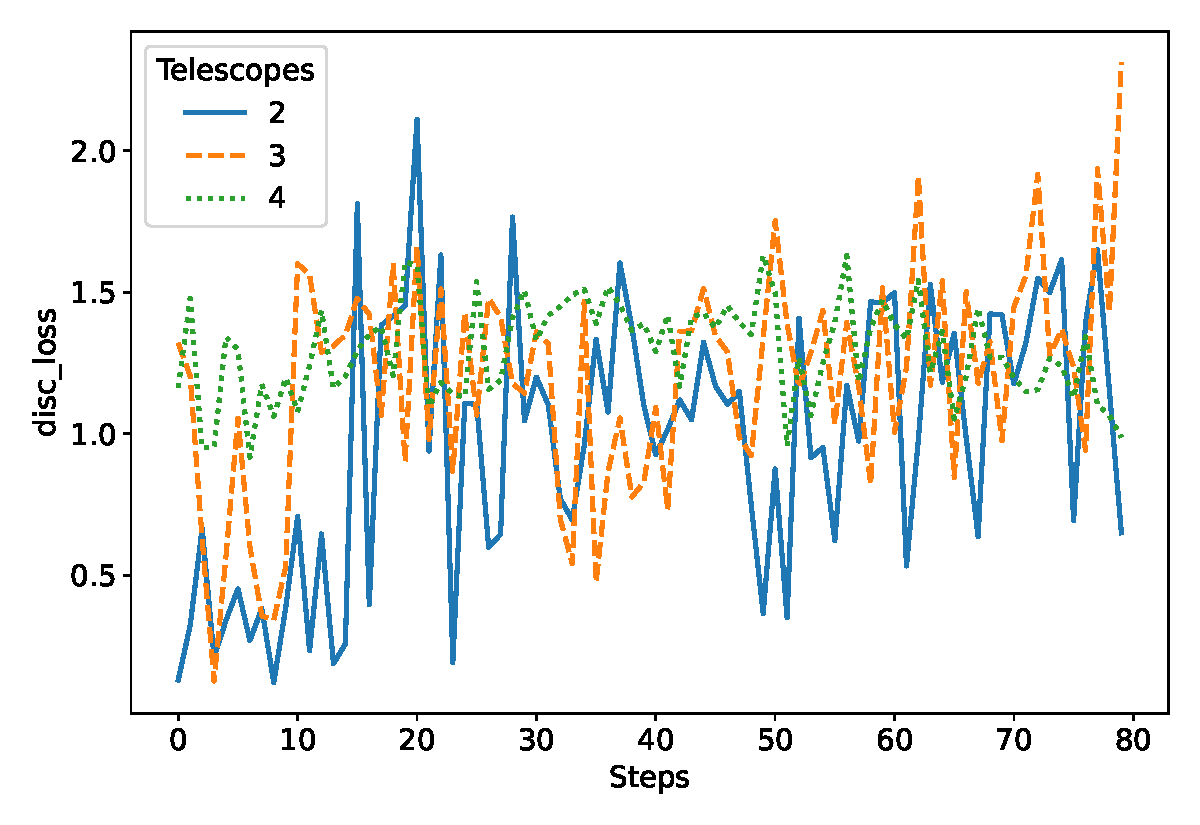
\includegraphics[width=\textwidth]{fig/analysis/Plot_N_telescopes_disc_loss.pdf}
		\caption{Discriminator loss for different amounts of telescopes.}
		\label{fig:Plot_telescopes_discloss}
	\end{subfigure}\hfill
	\begin{subfigure}{0.5\linewidth}
		\centering
		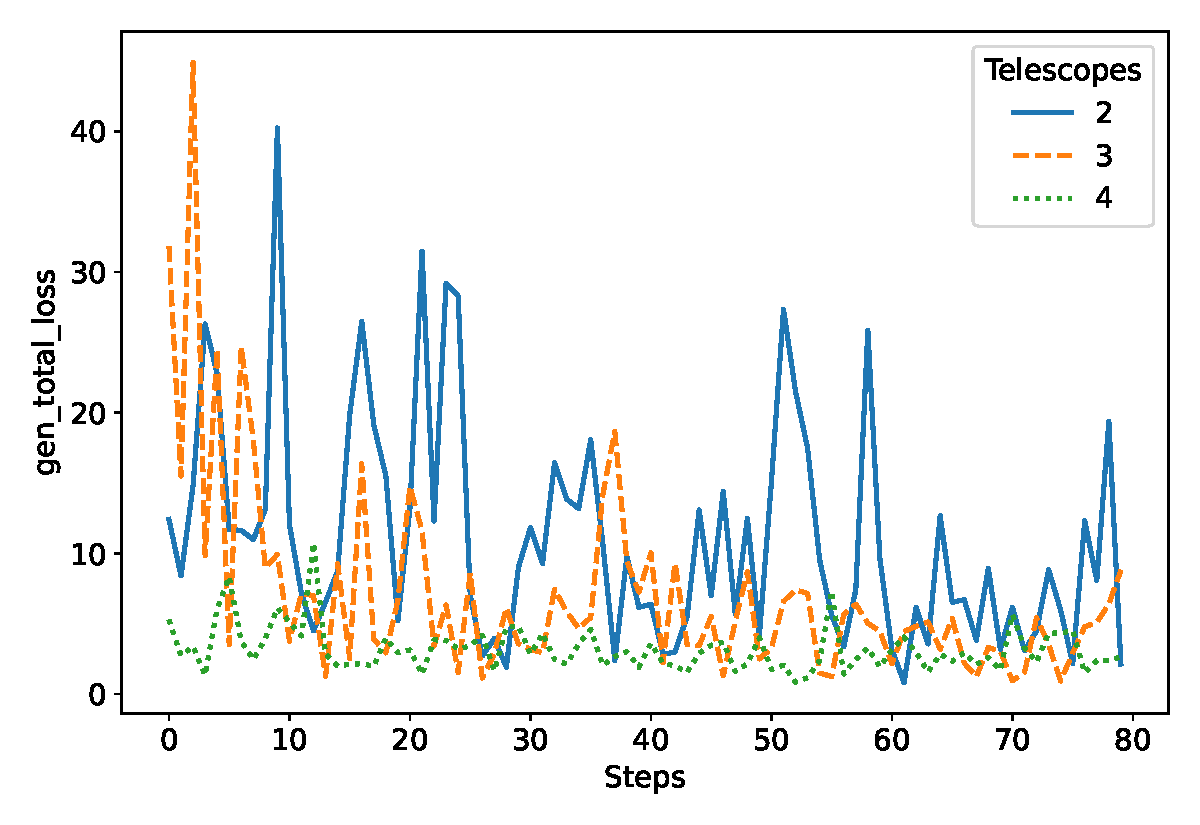
\includegraphics[width=\textwidth]{fig/analysis/Plot_N_telescopes_gen_total_loss.pdf}
		\caption{Generator loss for different amount of telescopes.}
		\label{fig:Plot_telescopes_genloss}
	\end{subfigure}\hfill
	\caption{The number of telescopes has a very impact on the model performance. If there are only two telescopes (1 baseline), both discriminator and generator are not trained smoothly: One gains a big advantage over the other. The result of four telescopes (6 baselines) is a lot better because the loss functions change only slightly with increasing steps.}
	\label{fig:Plot_telescopes_loss}
\end{figure*}
GANs can be extended to a conditional model \citep{mirza2014conditional}. In this case, both generator and discriminator receive extra information $y$, such that the value function of the conditional GAN (cGAN) can be expressed as:
\begin{equation}
	\centering
	\begin{aligned}
		V(D, G) &= \mathbb{E}_{x \sim p_{data}(x)} \left[ \log D(x|y) \right] \\
		&+ \mathbb{E}_{z \sim p_{z}(z)} \left[ \log \left( 1-D(G(z|y) \right) \right]
	\end{aligned}
	\label{eq:conditional_GAN}
\end{equation}

Furthermore, \citep{isola2017image} observed that combining the cGAN given in equation \ref{eq:conditional_GAN} with the traditional L1-loss improves results, as the generator tries to be close to the ground truth. Hence, the function that is minimized as:
\begin{equation}
	\centering
	L_{tot} = \arg \min_{G} \max_{D} V(D, G) + \lambda \cdot L_1(G)
	\label{eq:total_gen_loss}
\end{equation}
where $\lambda$ = 100 and $L_1(g)$ is given by equation (\ref{eq:l1_loss})
\begin{equation}
	\centering
	L_1(g) = \mathbb{E}_{x,y,z} \left[ ||{y - G(x,z)}||_1 \right]
	\label{eq:l1_loss}
\end{equation}

This type of network is shown to be very robust, as it has been applied to several problems. Examples include creating colored images from grayscale images, creating images of facades based on architectural labels, changing from day to night in different pictures, and predicting a map based on satellite data. A longer list of applications is given in \citep{isola2017image}. 


\subsection{Generator}
The used generator in this paper is a common U-Net convolutional network \citep{ronneberger2015u}. It consists of a contracting part, reducing the image size, and an expansive part, where the image is enlarged. The contracting part consists of repeated application of alternating convolutional layers and rectified linear unit (ReLU) layers. The expansion consists of repeated convolution, batch normalization, and ReLU layers. The first contracting step also includes a dropout layer \citep{isola2017image} 

\subsection{Discriminator}
The discriminator that has been taken here, named PatchGAN, does not work globally but rather classifies single patches as real or fake. The overall result is then estimated based on the average. The model architecture is as follows: zero padding, convolution, batch-norm, ReLu, zero-padding, and convolution \citep{isola2017image}.
\section{The Parameter Analysis for GAN}
\begin{figure*}
	\centering
	\begin{subfigure}{\linewidth}
		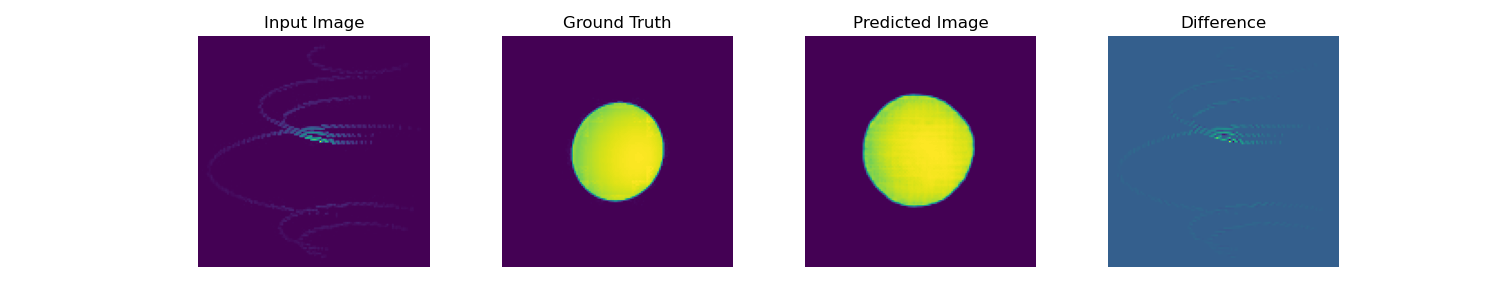
\includegraphics[width=\linewidth]{fig/testing_image/image_0.png}
	\end{subfigure}
	\begin{subfigure}{\linewidth}
		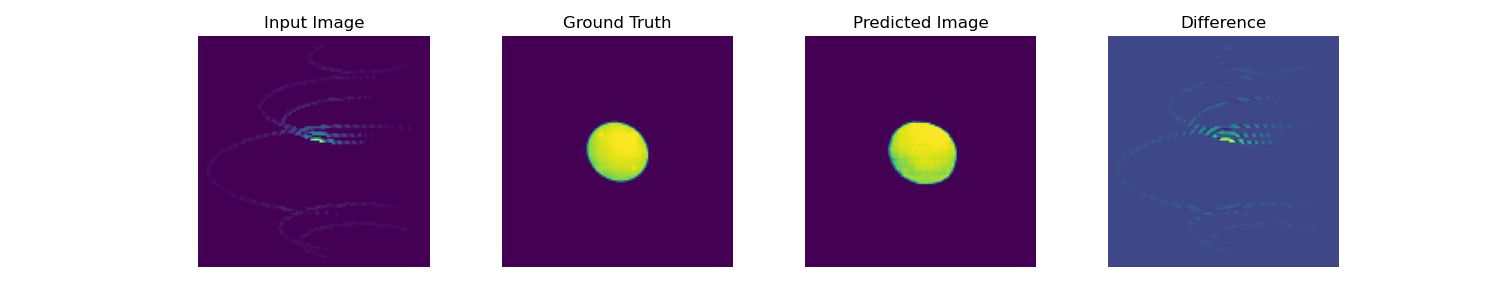
\includegraphics[width=\linewidth]{fig/testing_image/image_16.png}
	\end{subfigure}
	\begin{subfigure}{\linewidth}
		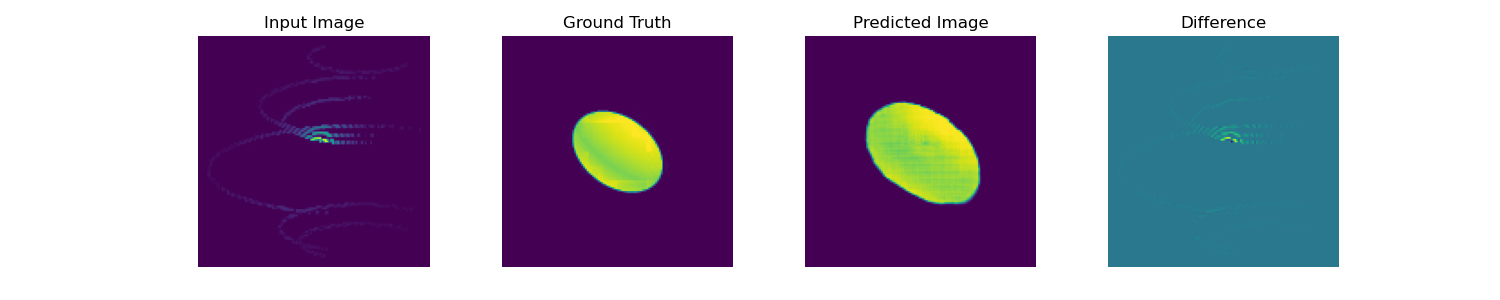
\includegraphics[width=\linewidth]{fig/testing_image/image_35.png}
	\end{subfigure}
	\begin{subfigure}{\linewidth}
		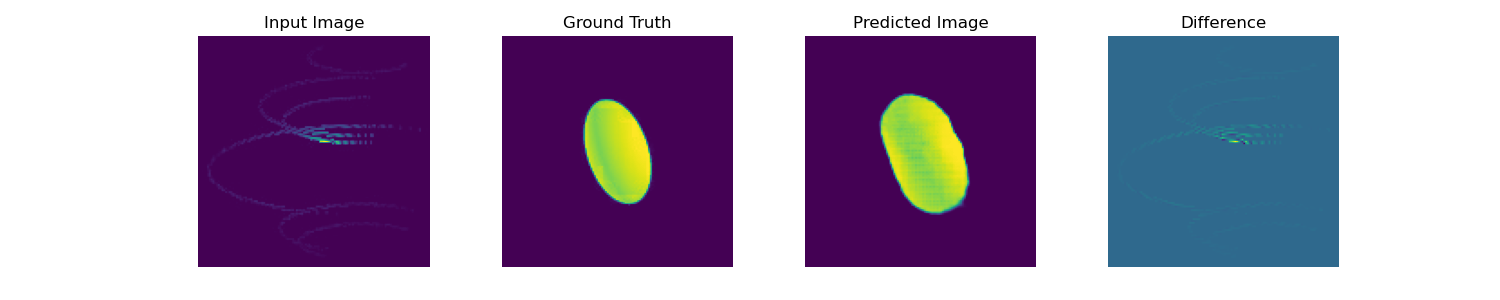
\includegraphics[width=\linewidth]{fig/testing_image/image_38.png}
	\end{subfigure}
	\begin{subfigure}{\linewidth}
		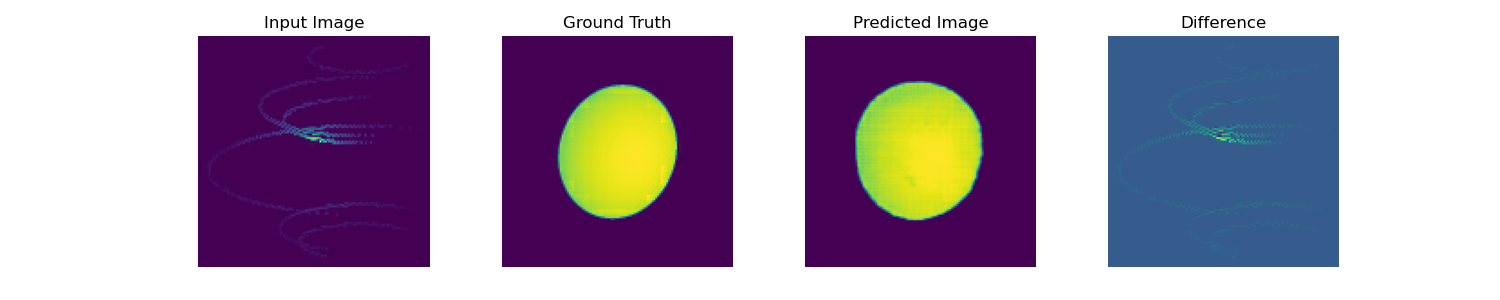
\includegraphics[width=\linewidth]{fig/testing_image/image_42.png}
	\end{subfigure}
	\begin{subfigure}{\linewidth}
		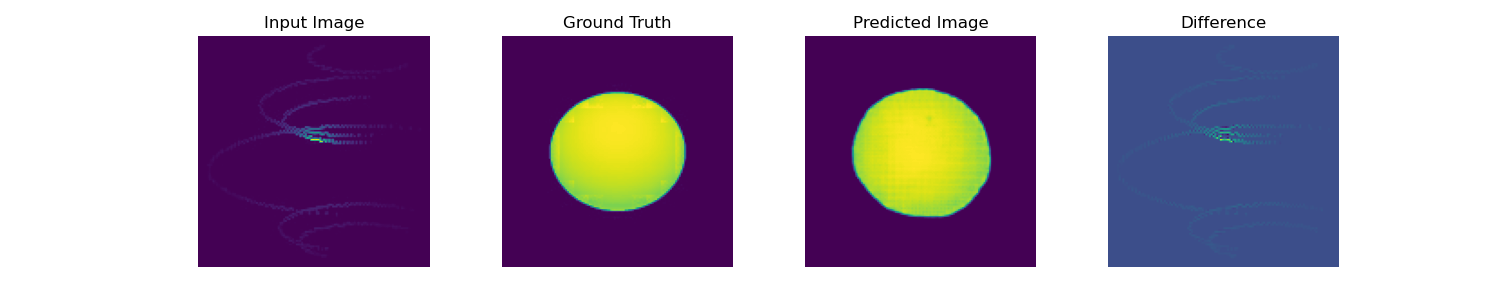
\includegraphics[width=\linewidth]{fig/testing_image/image_47.png}
	\end{subfigure}
	\caption{This set of figures shows the result of GAN for II. The left panels are signals using six baselines, which work as input for GAN. The first middle panel is the real image, also called ground truth, and GAN tries to mimic it during the training. The second middle panel is the reconstructed image, also called the predicted image, with trained GAN, and the end panel is the difference between the ground truth and the predicted image.}
	\label{fig:GAN}
\end{figure*}
Here, we discuss the parameters for the GAN structure, which is trained to reconstruct the image of stellar objects using II. Due to the adversarial nature of GAN, where the generator and discriminator compete in a min-max game, careful tuning of key parameters ensures that both networks are in good term to train the model.

\subsection{Data preparation}
First, we simulate fast-rotating stars, which are modeled as oblate spheroids with different radii and oblateness between 0.5 and 1. Different viewed angles have also been considered, with the effect of gravity darkening being linear dependence. The traced ellipses arise when integrating over the hour angle of the source. For the hyperparameter tuning and comparison of different telescopes, the total hour angle is about 11.5 hours. The ellipses are plotted and converted into grayscale images, resized, and stored as pure arrays to simplify further analysis. 
\begin{figure*}
	\centering
	\begin{subfigure}{0.33\linewidth}
		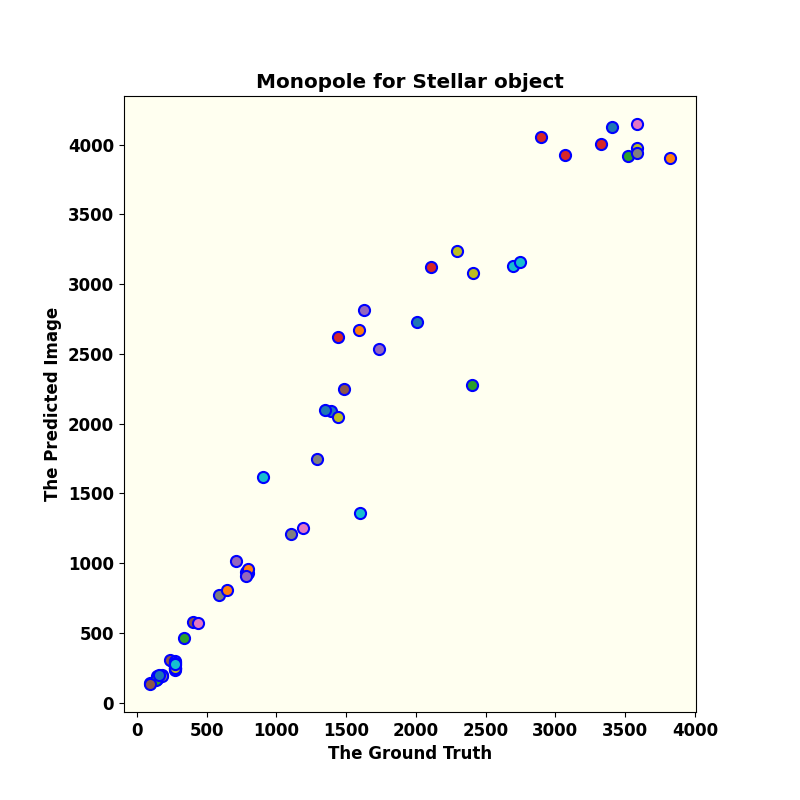
\includegraphics[width=\linewidth]{fig/moments/mom0.png}
		\caption{The monopole.}
		\label{fig:mom1}
	\end{subfigure}\hfill
	\begin{subfigure}{0.33\linewidth}
		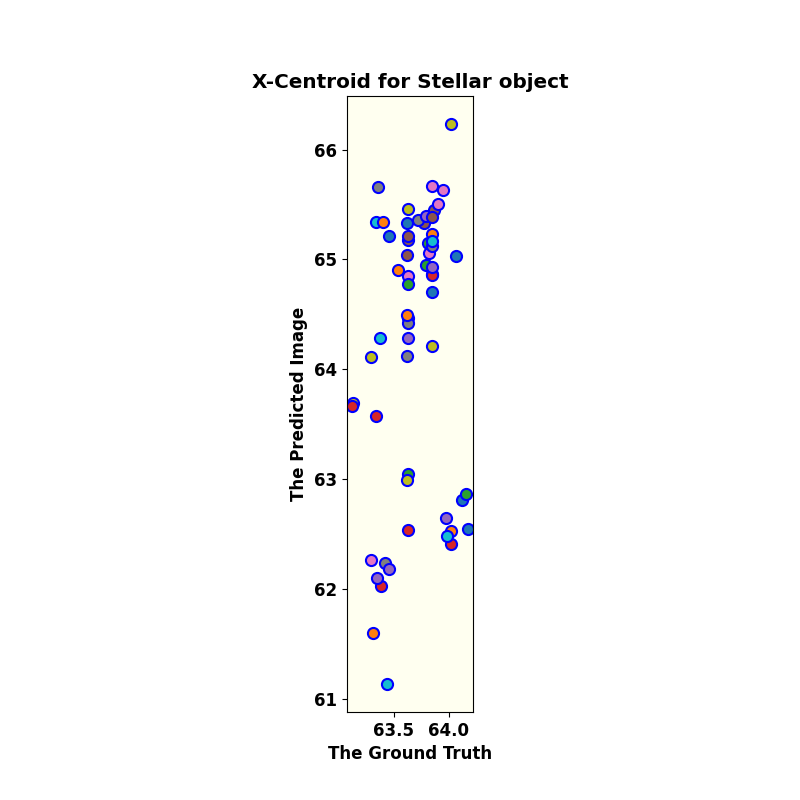
\includegraphics[width=\linewidth]{fig/moments/mom1.png}
		\caption{The centroids along x direction.}
		\label{fig:mom2}
	\end{subfigure}\hfill
	\begin{subfigure}{0.33\linewidth}
		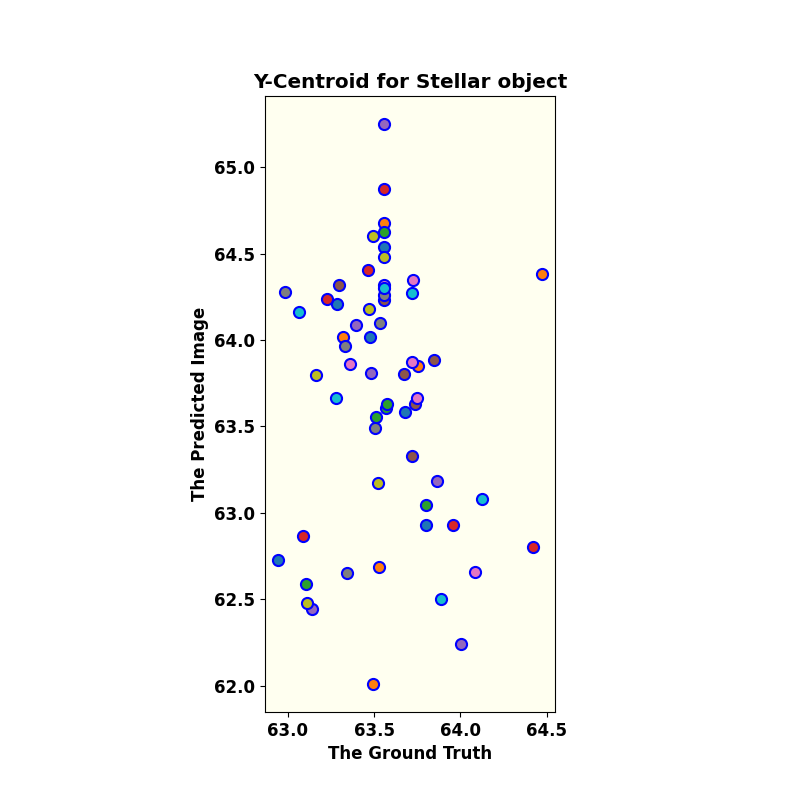
\includegraphics[width=\linewidth]{fig/moments/mom2.png}
		\caption{The centroids along y direction.}
		\label{fig:mom3}
	\end{subfigure}\hfill
	\caption{This set of figures shows the comparison of monopole, x-centroid, and y-centroid for ground truth and predicted images generated by trained GAN.}
	\label{fig:cen}
\end{figure*}
\begin{figure*}
	\centering
	\begin{subfigure}{0.33\linewidth}
		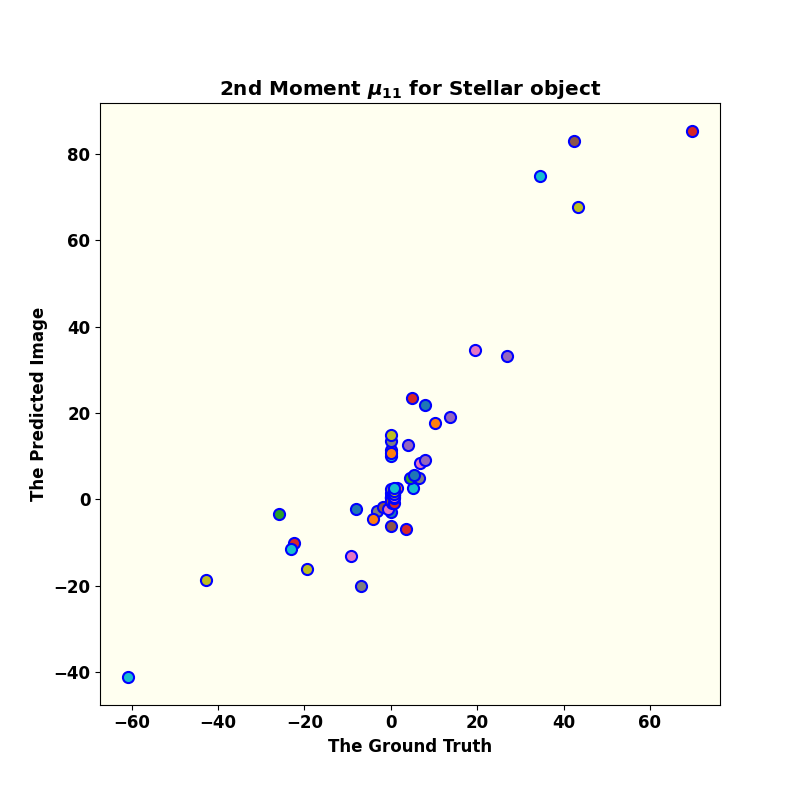
\includegraphics[width=\linewidth]{fig/moments/mom3.png}
		\caption{The 2nd order moment $\mu_{11}$.}
		\label{fig:mom4}
	\end{subfigure}\hfill
	\begin{subfigure}{0.33\linewidth}
		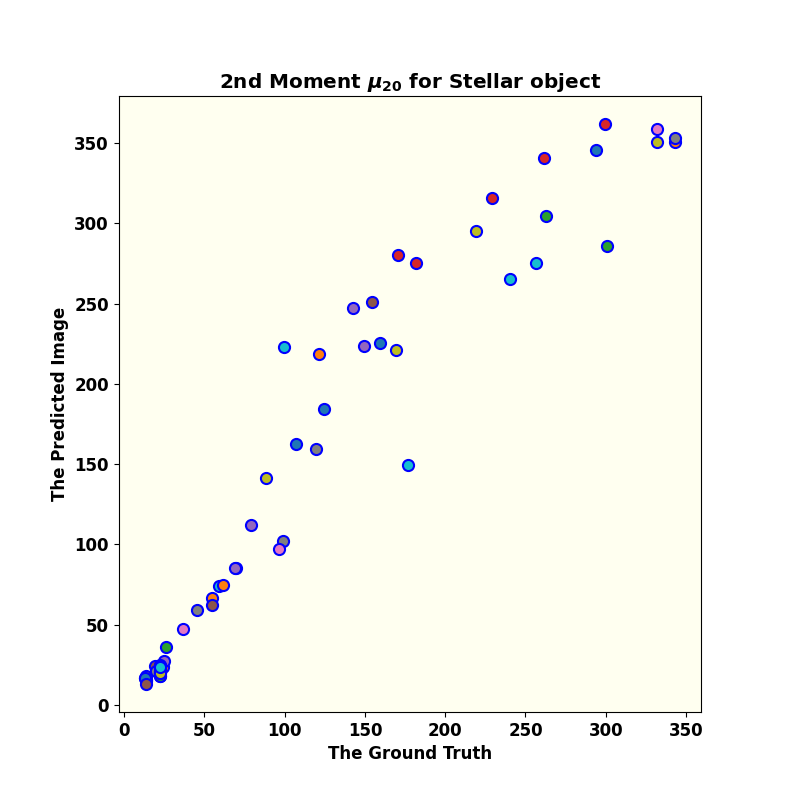
\includegraphics[width=\linewidth]{fig/moments/mom4.png}
		\caption{The 2nd order moment $\mu_{20}$.}
		\label{fig:mom5}
	\end{subfigure}\hfill
	\begin{subfigure}{0.33\linewidth}
		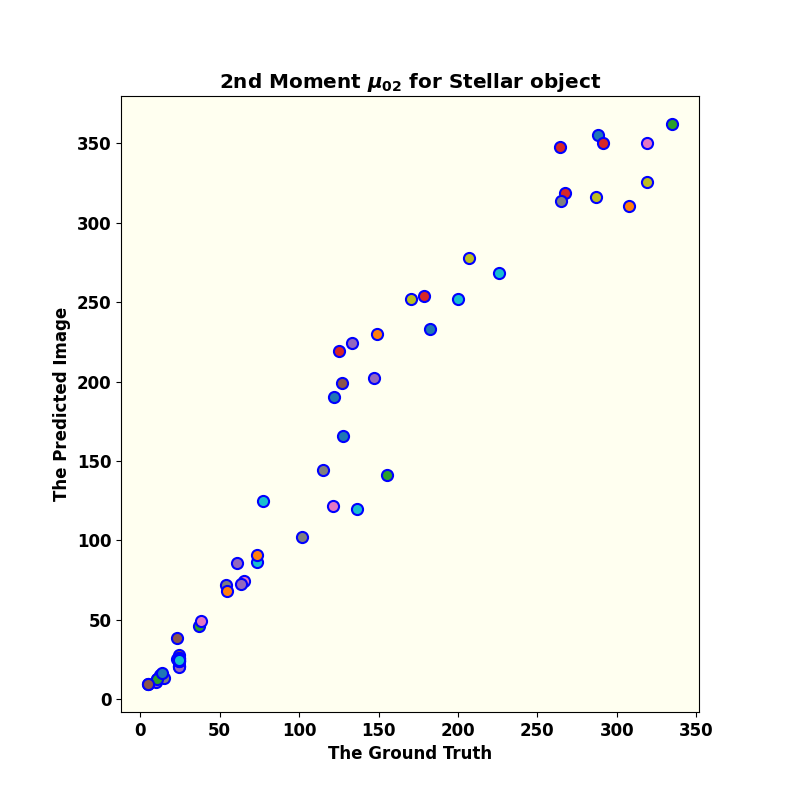
\includegraphics[width=\linewidth]{fig/moments/mom5.png}
		\caption{The 2nd order moment $\mu_{02}$.}
		\label{fig:mom6}
	\end{subfigure}\hfill
	\caption{The second-order central moments provide information about the size and shape of stellar objects. This set of figures shows all the second-order central moments for ground truth and predicted images generated by trained GAN.}
	\label{fig:struc}
\end{figure*}
\begin{figure*}
	\centering
	\begin{subfigure}{0.50\linewidth}
		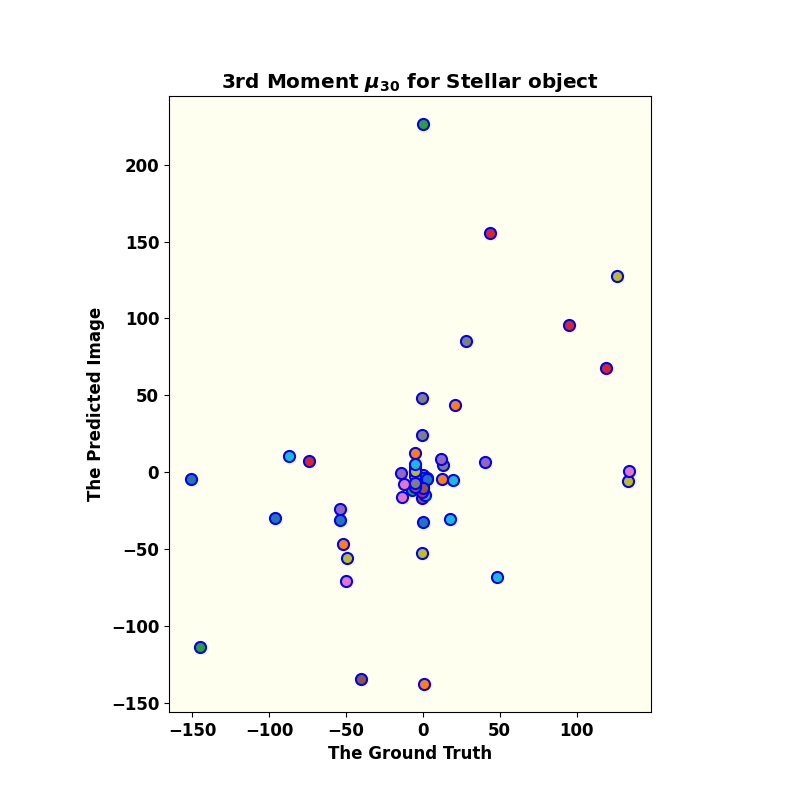
\includegraphics[width=\linewidth]{fig/moments/mom6.png}
		\caption{The 3rd order moment $\mu_{30}$.}
		\label{fig:mom7}
	\end{subfigure}\hfill
	\begin{subfigure}{0.50\linewidth}
		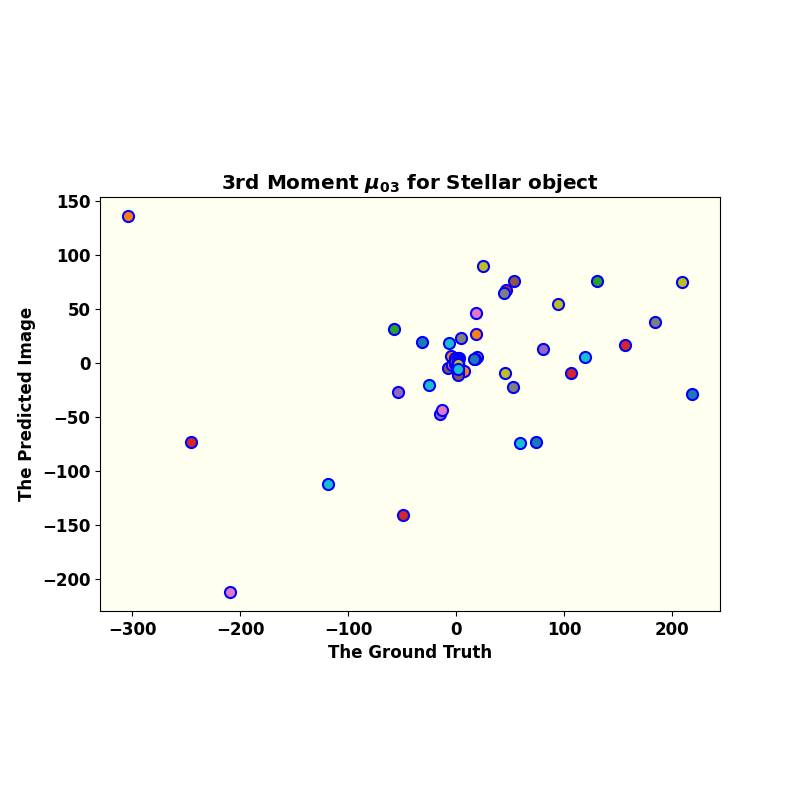
\includegraphics[width=\linewidth]{fig/moments/mom7.png}
		\caption{The 3rd order moment $\mu_{03}$.}
		\label{fig:mom8}
	\end{subfigure}\hfill
	\begin{subfigure}{0.50\linewidth}
		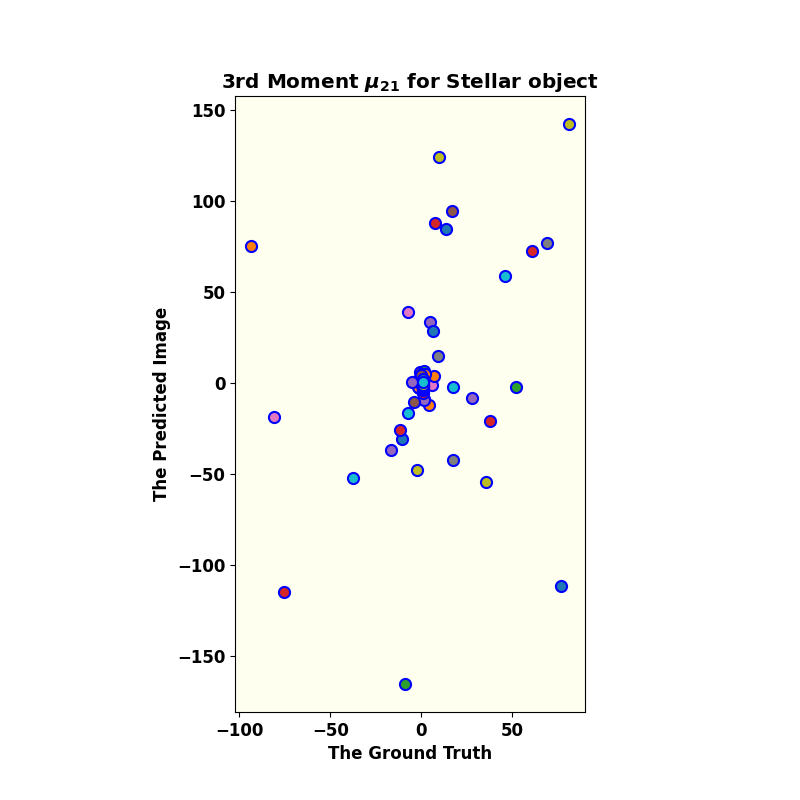
\includegraphics[width=\linewidth]{fig/moments/mom8.png}
		\caption{The 3rd order moment $\mu_{21}$.}
		\label{fig:mom9}
	\end{subfigure}\hfill
	\begin{subfigure}{0.50\linewidth}
		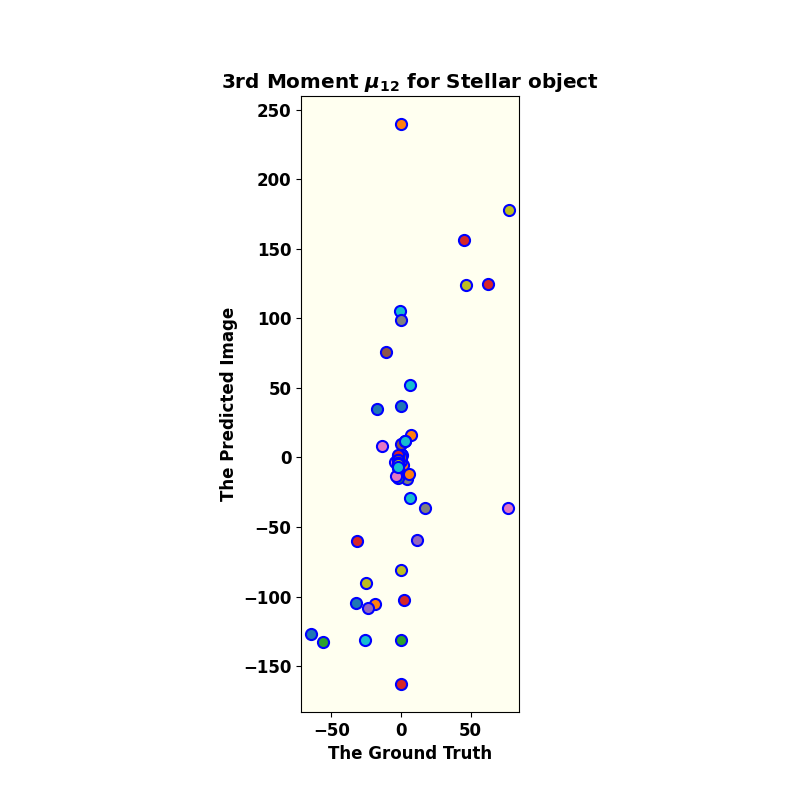
\includegraphics[width=\linewidth]{fig/moments/mom9.png}
		\caption{The 3rd order moment $\mu_{12}$.}
		\label{fig:mom10}
	\end{subfigure}\hfill
	\caption{This set of figures shows all the 3rd-order central moments for ground truth and predicted images generated by trained GAN. It calculates the skewness and evaluates the brightness distribution of images.}
	\label{fig:moments}
\end{figure*}

First, Salt and Pepper noise is introduced at a rate of $\alpha$ (usually 0.5\%). Then, the images are resized, and the mean is subtracted. A two-dimensional Fast Fourier Transform, as well as a Fourier shift, is applied, which yields a complex number of every pixel. As II does not measure the phase, the absolute value is calculated (shown in Fig.~\ref{fig:ft} on a linear and logarithmic scale for visualization). The sparse sampling is also introduced, namely by a pixel-wise multiplication between the absolute valued Fourier transformed image and the sparse sampling map. The result is a map in the Fourier plane with several ellipses, also called the sparse sampling map. Fig.~\ref{fig:ft_base} shows the sparse sampling for Fig.~\ref{fig:image} as the source with four telescopes (Fig.~\ref{fig:teles}). Finally, the pixels are normalized and converted to 8-bit integers. This image represents the sparsely sampled complex visibility, as it can be measured with II. The image shown in Fig.~\ref{fig:ft_base} is the input image for the GAN, which also requires the ground truth image. So, the simulated stars are also resized using the same algorithm and converted to 8-bit integers to reduce the bias. The GAN must know the ground truth corresponding to an input image. Hence, they are merged side-by-side, shown in Fig.~\ref{fig:GANinput}, and used as input to train the GAN. This procedure is conducted for all the simulated stars, with 10\% acting as test data, 10\% as validation data, and the remaining 80\% as training data. 

\subsection{GAN architecture}
The GAN used in this work is based on pix2pix \citep{isola2017image}, which uses a cGAN discussed in the last section. It is very robust and could already be applied to various problems. An example can be found in the TensorFlow tutorials\footnote{\url{https://www.tensorflow.org/tutorials/generative/pix2pix}}, where it is applied to a data set of architectural facades. However, to adapt the pix2pix GAN for the phase retrieval problem, some modifications are necessary. The network uses the TensorFlow \citep{abadi2016tensorflow} library, calculations are performed with scipy \citep{virtanen2020scipy}, and plots are drawn with matplotlib \citep{4160265}.
\begin{figure*}
	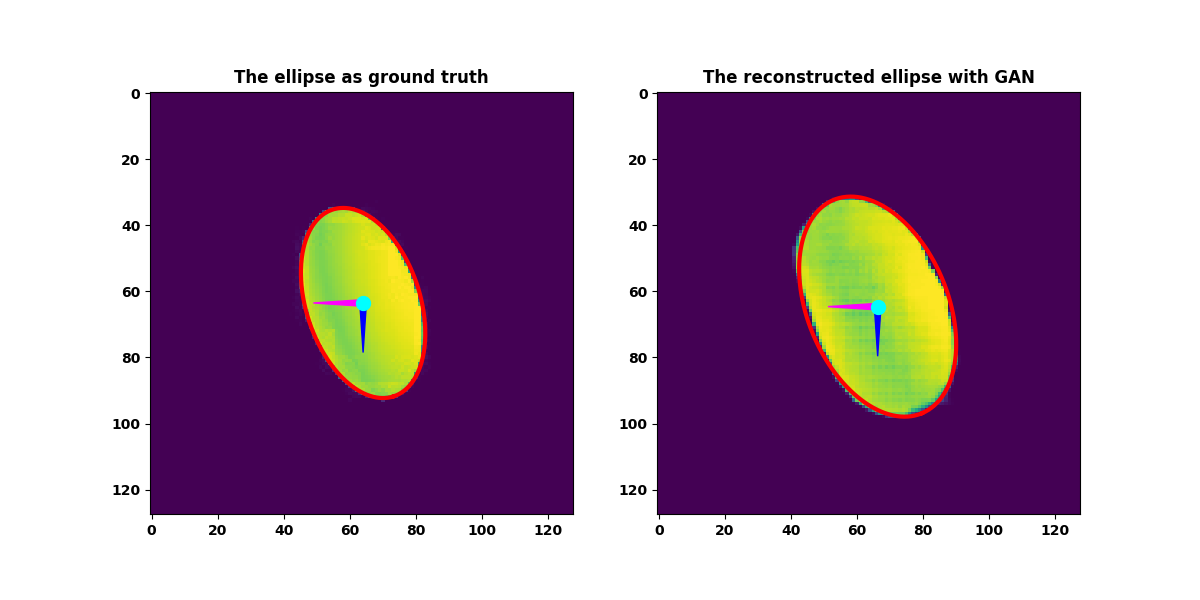
\includegraphics[width=\linewidth]{fig/reconstruction.png}
	\caption{The elliptical image of ground truth and predicted image by trained GAN. The elliptic curve (in red) was drawn using the second-order moment, and cyan dots show the centroids (mx, my) of the images. There are two arrows in each image showing the skewness of pixel distribution along the x and y axes (magenta and blue color).}
	\label{fig:recons}
\end{figure*}
\subsection{Hyperparameter tuning}
The GAN used for this work depends on several parameters, which will be explained here briefly (an in-depth discussion can be found in \citep{murphy2022probabilistic}).

The learning rate of the optimizer is a measure of how much the model changes per iteration. Small learning rates can lead to underfitting, and large learning rates can make the model unstable. It is therefore important to carefully choose the learning rate \citep{murphy2022probabilistic}. Fig.~\ref{fig:Plot_learning_rate_loss} shows the effect of the learning rate on both generator and discriminator loss for three different values of it. Both loss functions have fewer outliers with decreasing learning rates, which is expected, as there is less change in the models with low learning rates. Even though all models stabilize at the same level, low learning rates are preferred.

The kernel size is the size of the kernel in the convolutional layer. It determines the amount of pixels that are linearly combined into a new pixel. A large kernel size allows one to catch features that are a few pixels away, but it also means that unrelated features might be introduced. The kernel size does not have a big effect on the loss functions, as shown in Fig.~\ref{fig:Plot_kernel_size_loss}. Smaller kernel sizes seem to have more outliers, which means that either generator or discriminator gains an advantage. Therefore, a kernel size of 5 is preferred.

The amount of noise is reflected by the two parameters $\alpha$ and $\beta$. Both indicate the percentage of pixels that change to either black or white, hence the name Salt and Pepper noise, where $\alpha$ is introduced in the real image, $\beta$ in the generated image. Different ratios $\frac{\alpha}{\beta}$ can lead to different model performances. There is no significant difference between distinct noise rates introduced in the images. Fig.~\ref{fig:Plot_noise_loss} shows the loss functions on smaller images (64 x 64). As there is no effect, it was not necessary to repeat this analysis for larger images. 

The batch size defines the number of images that pass the network simultaneously. It is observed that smaller batch sizes can lead to better generalization \citep{prince2023understanding}. Fig.~\ref{fig:Plot_batchsize_loss} shows two different batch sizes. Here, when two images are processed simultaneously, there are fewer outliers, but since it increases the training time heavily, a batch size of 1 is used.

While training GAN, one can give the discriminator an advantage by increasing the number of training steps before returning to the generator training. It can increase the performance of the model. However, it increases the training time as well and leads to a lower discriminator loss score, as shown in Fig.~\ref{fig:Plot_discrep_loss}. At the same time, the generator score increases slightly, which should be no surprise. Because the generated images did not improve with higher discriminator training, they are usually trained in the same amount as the generator.

Finally, the amount of sparse sampling can be varied, giving the model access to more pixels. More telescopes automatically lead to more baselines and, hence, more pixels that are available. Fig.~\ref{fig:Plot_telescopes_loss} shows the loss functions for different numbers of telescopes. There is a huge disparity, which can partly be explained by the fact that the relation between telescopes and baselines is not linear. The Fourier plane can be sampled sixfold when using four telescopes in contrast to only two telescopes. In the latter case, both the generator and discriminator are not trained smoothly, as seen by the outliers. It is already better with three telescopes and very promising when using four telescopes. The degree of sparse sampling seems to have the biggest effect of all hyperparameters.
\section{The Reconstructed Image with GAN}
In this section, we will first discuss phase retrieval using hyperparameters, as mentioned earlier, followed by an analysis where multiple sources are trained simultaneously. The best performance for image reconstruction has been observed with a learning rate of $2 \cdot 10^{-4}$, a kernel size of 5x5, and equal noise percentages in original and generated images. The batch size selected is 1, and the discriminator-generator receives equal training.
\subsection{The Predicted Image with Trained GAN}
The success of the GAN in training the model for Intensity Interferometry to reconstruct images of fast-rotating stars is demonstrated in Fig.~\ref{fig:GAN}. The GAN was trained on training datasets for 60,000 steps. After training, the GAN was tested on different validation datasets, producing predicted images of a fast-rotating star. Fig.~\ref{fig:GAN} presents a set of four combined images demonstrating the GAN's performance in reconstructing the shape, size, and brightness distribution of the fast-rotating star using II. The left panel shows the signals covered by six baselines, which serve as the input for the generator to train the GAN. The first middle panel displays the real image, or ground truth, which the discriminator uses to differentiate between real and generated images from the generator. During training, the GAN aims to mimic this ground truth. The second middle panel depicts the reconstructed image, or predicted image, produced by the trained GAN. This panel illustrates the success of the GAN in image reconstruction using II. The right panel shows the difference between the ground truth and the predicted image. This difference should be minimized for high-precision image reconstruction with the application of GAN on II. The predicted images of Fig.~\ref{fig:GAN} showed positive results, accurately providing visual information about the source's size and shape, as well as the distributed brightness. This image reconstruction was achieved using only six baselines. However, the results can be further improved by increasing the number of telescopes to cover more (u, v) planes, making the existing and upcoming Cherenkov Telescope Array Observatory (CTAO) an ideal candidate in collaboration with existing CTA. 
\subsection{Evaluation of GAN using moments}
After the success of GAN in reconstructing the image using II, there is a need for evaluation of it. So, we use the image moments. Image moments are statistical properties that provide information about the reconstructed shape, size, and intensity distribution of the objects in the image. These moments help quantify key features like the position, orientation, and distribution of brightness in the image, allowing for an objective evaluation of how well the predicted image corresponds to the actual object. We will analyze the consistency and accuracy of the GAN-generated image by comparing its moments to those of the ground truth. It provides a reliable framework for evaluating reconstruction quality, as image moments highlight the subtle differences in geometric and intensity properties that might not be visually apparent. 

The raw moment $M_{ij}$ of an image I(x, y) is defined as \citep{hu1962visual}
\begin{equation}
	M_{ij} = \sum_{x} \sum_{y} x^i y^j I(x, y).
	\label{eqn:Mom}
\end{equation}

The zeroth order raw moment, which is the total intensity of an image and is called the monopole. It sums up all the pixel values across the image, providing an overall intensity value. So, the study of monopole provides the total flux of fast-rotating stars here. According to eqn.~\ref{eqn:Mom}, the monopole of a image is calculated as 
\begin{equation}
	M_{00} = \sum_{x} \sum_{y} I(x, y).
\end{equation}
Fig.~\ref{fig:mom1} shows the monopole for 50 different reconstructed images. It shows the linear behavior for the monopole between the ground truth (the real image) along the x-axis and the predicted image (reconstructed image) along the y-axis, which is obvious for different shape-size sources. This result explains the similarity between the total intensity of both images. It ensures that the predicted image has the approximately correct total brightness (the flux) compared to the ground truth. However, monopole does not explain the shape, size, and brightness distribution of fast-rotating stars. So, there is a need for higher-order moments.

The center of mass for the fast-rotating star or any other stellar object is calculated using the centroid (in x and y directions). These centroids are given in terms of first-order raw moment and monopole as
\begin{equation}
	\begin{aligned}
		&m_x = \frac{\sum_{x} x I(x,y)}{\sum_{x} \sum_{y} I(x, y)} = \frac{M_{10}}{M_{00}} \\
		&m_y = \frac{\sum_{y} y I(x,y)}{\sum_{x} \sum_{y} I(x, y)} = \frac{M_{01}}{M_{00}}
	\end{aligned}  
\end{equation}
Fig.~\ref{fig:mom2} and Fig.~\ref{fig:mom3} show the comparison of centroid along the x and y axis for 50 predicted images with respect to ground truths. The clustering of centroids in a given scale range for all the results explains that the reconstructed image correctly represents the spatial location of the fast-rotating star in compare with the ground truth.

Further, these calculated centroids will help to study the shape, size, and brightness distribution of fast-rotating stars in terms of higher-order image moments. For that, the central moment of an image is calculated according to
\begin{equation}
	\mu_{pq} = \frac{1}{M_{00}}\sum_{x} \sum_{y} (x - m_x)^p (y - m_y)^q I(x, y).
\end{equation}
The sum of $p$ and $q$ defines the order of the central moment.

The second order central moment ($\mu_{11}, \mu_{20}, \mu_{02}$) has been shown in Fig.~\ref{fig:struc}, which is used to study the structure of a fast-rotating star along the line of sight of observation (explain in upcoming subsection). All these three plots explain the linear relation of second-order moments again as for monopole and show the success of the application of GAN to reconstruct the image with II.

The information on brightness distribution is gathered using the skewness of the image by calculating third-order central moment ($\mu_{30}, \mu_{03}, \mu_{21}, \mu_{12}$) of images. Fig.~\ref{fig:moments} shows all third-order moments for the ground truth and reconstructed image. The skewness along the x and y axis ($\mu_{30}, \mu_{03}$) to test the GAN for II are acceptable, which can be seen in Fig.~\ref{fig:mom7} and Fig.~\ref{fig:mom8}, where a linear relation exists between ground truth and predicted image. However, the remaining higher moments $(\mu_{21}, \mu_{12})$ shown in Fig.~\ref{fig:mom9} and Fig.~\ref{fig:mom10} are not in good terms specially $\mu_{12}$.

\subsection{The reconstructed Parameters for object}
The centroids $(m_x, m_y)$ represents the center of the fast-rotating star. However, the calculated second-order central moment defines the orientation, semi-major axis, and eccentricity of the source \citep{teague1980image}. These parameters fully describe the ellipse that fits the image data based on the moments. 

The orientation along the line of sight is defined as
\begin{equation}
	\theta = \frac{1}{2}\arctan \big(\frac{2\mu_{11}}{\mu_{20} - \mu_{02}}\big).
	\label{eqn:orn}
\end{equation}
The semi-major and semi-minor axis will be calculated according to
\begin{equation}
	\begin{aligned}
		&a = 2\sqrt{mp + \delta} \\
		&b = 2\sqrt{mp - \delta}
	\end{aligned}
	\label{eqn:semi}
\end{equation}
where,
\begin{equation}
	mp = \frac{\mu_{20} + \mu_{02}}{2}
	\label{eqn:mp}
\end{equation}
and
\begin{equation}
	\delta = \frac{\sqrt{4\mu_{11}^2 + (\mu_{20} - \mu_{02})^2}}{2}.	
	\label{eqn:delta}
\end{equation}
So, the eccentricity of the fast-rotating star in terms of axis value is 
\begin{equation}
	e = \sqrt{1 - a/b}.
	\label{eqn:eccen}
\end{equation}
Fig.~\ref{fig:recons} shows all zeroth to third order moments only for one ground and predicted image. In this figure, there is a red curve for both ground truth and predicted image, which is the representation of all second-order moments in terms of eqn.~\ref{eqn:orn} to eqn.~\ref{eqn:eccen} as orientation, axis value, and eccentricity. There is a cyan dot point as well, which represents the zeroth order moment for both images. There is also a third-order moment, which is expressed in terms of arrows in magenta and blue color to view the skewness along the x and y axes.
\section{Conclusion}
Intensity Interferometry (II), a technique, is emerging after a long gap to overcome the challenges of Amplitude Interferometry with optical wavelength range. It is rejuvenated with support from advanced facilities at the Imaging Cherenkov Telescope Arrays (ICTAs). These telescopes are instrumental in capturing high-resolution images equipped with large aperture areas and sensitive photon detectors (capable of resolving signals within a nanosecond) \cite{dravins2013optical}. The Major Atmospheric Gamma Imaging Cherenkov Telescope (MAGIC), one of the CTA in the world, is now being used for II, observing stellar objects with its 17-meter diameter mirror \cite{lorenz2004status}. The telescope has already demonstrated the potential of II by measuring and comparing the diameters of individual stars \cite{abe2024performance}. Other existing arrays (Very Energetic Radiation Imaging Telescope Array System (VERITAS) and High Energy Stereoscopic System (HESS)) are also making progress as II when gamma-ray observation stops \cite{kieda2021veritas, zmija2022optical}. Future observations, made possible by more advanced, sensitive instrumentation and upcoming CTAO, promise to push the boundaries of what we can observe with optical range. However, there is a drawback of II in terms of phase loss of signal, capturing only its magnitude via photon correlation. Here, the challenge of phase retrieval in II has been effectively addressed through the application of machine learning techniques, particularly with conditional Generative Adversarial Networks (cGAN). Our study demonstrates that the application of cGAN on II data successfully recovers the size, shape, and brightness distribution of a fast-rotating star. The evaluation based on image moments, specifically the monopole, second, and third-order moments, supports the effectiveness of the cGAN in achieving accurate image reconstruction from a one-night simulation of II using six baselines. A critical factor in the performance of the reconstruction process is the extent of Fourier plane coverage, which is determined by the number of available telescopes and the total observing time. The brightness distribution can likely be reconstructed with even higher precision with a full night of observation using four telescopes. Future work could explore different observatory layouts to study the impact on image reconstruction quality, such as the Southern Cherenkov Telescope Array (CTA) with MAGIC.

While the results of this study demonstrate the significant potential of machine learning, particularly cGAN, for image reconstruction in II, several aspects need further refinement. (1) Detector efficiencies, which impact the signal-to-noise ratio (SNR) of real observational data, have yet to be incorporated. It will be crucial to address these challenges for more accurate SNR estimation. Incorporating these efficiencies in future work will be important for providing a more accurate estimate of the SNR. (2) Exploring and comparing different methods to generate images, which works better than cGAN to reconstruct stellar images with II. (3) Different loss functions can be used to check the reconstruction quality. So, there are further testing is required to refine the GAN and make it more robust and reliable. However, our findings suggest that machine learning is a promising approach for phase reconstruction in II.

In summary, though cGAN has shown promising results, further testing and improvements are necessary to make the model more robust and reliable in practical applications. Overall, this study highlights the potential of machine learning approaches for advancing phase retrieval and high-resolution image reconstruction in II, suggesting exciting future directions in the application of AI to optical astronomy.

\bibliographystyle{mnras}
\bibliography{refs.bib}

\end{document}